\chapter{Flow Cytometry Analysis}

Here we talk about flow cytometry data, how we analyze and visualize it; and how we use that analysis alongside with some machine learning tools to classify samples into cancer subtypes.

\section{Flow Cytometry}
Flow cytometry is a technology that allows measurement of biomarkers inside and outside cells on a single cell basis~\cite{flow-cytometry}. The technology can also sort and separate certain cells according to a given criterion~\cite{flow-cytometry-sorting}.

Cell preparation in flow cytometry involves suspension of the cells in a liquid containing biomarker reagents. Reagents are marked antibodies that can be detected by the laser beams in the flow cytometer machine~\cite{flow-cytometry-cell-preparation}. The antibodies are usually marked with a fluorescent label. Each fluorescent marker has a corresponding peak excitation and emission wavelength which can be detected using lasers or lamps available on the flow cytometer machine. The combination of markers has to be chosen such that their corresponding wavelengths have minimal overlap; otherwise they cannot be distinguished from one another due to interference between them.

In a flow cytometer cells flow in a liquid stream one by one, where a lamps or laser beams in conjunction with sensors measure the intensity of reflected light from the cells. These measurements can be in linear or logarithmic space~\cite{practical-flow-cytometry-book}. The measured values depend on the light intensity projected onto cells which can be tuned by changing the voltage of the lasers or lamps. Different wavelengths correspond to different markers, but they might overlap. When the tail of the emission spectrum of a marker overlaps with the main part of the emission spectrum of another marker, it is called spillover as shown in Fig.~\ref{fig:flow-cytometry-spillover}~\cite{flow-cytometry-compensation}.

Compensating for spillover requires a spillover matrix ($SM$). $SP_{i,j}$ shows the percentage that marker $i$ spills over marker $j$. The compensation matrix ($CM$) is then the calculated as the inverse of the spill over matrix. Let $S$ be the true signal value, and $O$ be the observed value. Then we have~\footnote{\url{http://bioinformin.net/cytometry/compensation.php}}:

\begin{align}
  &CM = SM^{-1} \nonumber \\
  &S = O \times CM
  \label{fml:fcs-compensation}
\end{align}

\begin{figure}[!ht]
  \centering
  \includegraphics[height=7cm]{figs/fcs-spillover}
  \caption{[DIRECT QUOTE] Fluorescence emission spectra for FITC and PE. The emission spectrum (the wavelengths of light generated by excitation of these molecules) is shown for an excitation at $488nm$ (the same as the argon-ion laser line). FITC emission is maximal at $\sim 515nm$; typically, a filter centered on $530nm$ is used to collect the emitted light (shaded region). The emission of is farther red, with a maximum at $\sim 575nm$; typically, a filter centered on this emission maximum is used to collect. Note that PE has some emission in the wavelength bands used to collect PE fluorescence (B); typically, the amount of light in the $575nm$ band is $\sim 15\%$ of that in the $530nm$ band (A). The PE has very little emission in the $530nm$ band (C), usually less than $2\%$ of the emission in the $575nm$ band (D)~\cite{flow-cytometry-compensation}.}
  \label{fig:flow-cytometry-spillover}
\end{figure}

\section{Data Preprocessing and Challenges}
Transformation and spillover compensation are the two main phases of raw flow cytometry data preprocessing.

\emph{Transformation}: The measured fluorescent intensities almost exponentially correspond to the number of existing fluorescent markers on or inside the cell. Therefor a proper transformation of the raw data is essential in order to have the data in a linear space. Logarithmic, log-linear hybrid transformation Logicle~\cite{fcs-logicle}, and hyperbolic arcsine~\cite{fcs-arcsineh} are some commonly used transformations. Some studies have compared different transformation techniques and reported their advantages and disadvantages~\cite{fcs-transformation-survey1, fcs-transformation-survey2}.

\emph{Spillover Compensation}: Compensation is done as shown in Formula~\ref{fml:fcs-compensation} and it relies on a given compensation or spillover matrix.

In practice data are produced through time and also maybe in different labs. This means reagent batches are different, and also flow cytometry machines are not necessarily calibrated alike, which also affects compensation matrices. Therefore normalization is a crucial step to make samples comparable~\cite{fcs-normalization}.

\section{High Dimensional Analysis and Visualization}
Manual analysis of flow cytometry data involves \emph{gating}. Researchers use density or scatter plots of one or two selected dimensions  of flow cytometry data in order to visualize and also select some areas on those plots to further investigate cells within the selected area. Visualization and further gating of those selected cells is commonly a next step to the analysis.

Manual gating of cells across several samples is a labor intensive and time consuming process. Not being able to analyze the data in its original higher dimensional space is another disadvantage of manual flow cytometry data analysis.


\subsection{flowType}
Flow cytometry has undergone a ``chromatic explosion'' over the past decade and can now measure 17 markers at once for each of hundreds of thousands of individual cells \cite{Chattopadhyay2008}.
Since then, mass cytometry has enabled measurement of 30--45 markers per cell \cite{Bendall2012a}, while single-cell multiplexed RT-qPCR can measure 50--96 mRNAs per cell \cite{White2011}. 
The growth in high-throughput single-cell data continues to outpace development of corresponding bioinformatics techniques \cite{Chattopadhyay2008}.
To answer this challenge, we previously developed flowType \cite{Aghaeepour2012} and RchyOptimyx \cite{Aghaeepour2012a}. 
flowType uses partitioning of cells, either manually or by clustering, into positive or negative for each marker to enumerate all cell types in a sample, e.g. \cite{Aghaeepour2013Critical}.
RchyOptimyx measures the importance of these cell types by correlating their abundance to external outcomes, such as disease state or patient survival, and distills the identified phenotypes to their simplest possible form. 
These packages have been used to identify several novel cell populations correlated with HIV outcome \cite{Aghaeepour2012}. 
More recently, this pipeline has been used to evaluate standardised immunological panels \cite{Villanovaa2013Computational}, to optimise lymphoma diagnosis \cite{Craig2013Computational}, and to analyse a range of other clinical data (unpublished).

However, the higher dimensionality of data produced by mass cytometry generates up to $3^{45}\approx10^{21}$ possible cell types, with an even greater number (up to $3^{96}\approx10^{45}$) for single-cell qPCR; these magnitudes are beyond the capabilities of flowType and RchyOptimyx.
Furthermore, flowType and RchyOptimyx have thus far only treated cells as being either positive or negative for a marker.
In practice, many biomarkers can have a range of expression levels such as ``dim'' and ``bright''. 
In this application note, we detail architectural improvements to flowType and RchyOptimyx to overcome these limitations.  
%
%
%
%RB
%\textbf{missing legend in panel C \& remove 12GB line in red as it looks like flowType-BF line, BF line in panel D?; y axis should be GB in panel C (who measure memory in bytes?), missing y axis marks in panel d and x and y-axis lines in d, fix gaps in lines for other panels where appropriate (b-x axis)  [for a 15 marker sample] this text not needed in legend in panel D I think)}
%
% Biggest thing is I save 5 lines of text by cutting white space out from top and bottom of figure, could probably save a few more as needed after you produce next (hopefully final) version. 
%
%
%
\begin{figure*}[!tpb]%figure1
\center{\includegraphics[width=\textwidth]{figs/flowtype2-figure}}
\caption{
\textbf{a-b. Run time comparison of flowType-DP to flowType-BF} in terms of number of cells (a) and number of markers (b). 
\textbf{c-d. Possible thresholds for marker combinations using flowType-DP} for typical mass cytometry data (c) and polychromatic flow cytometry data (d). 
\textbf{e-f. Three/four-partition flowType-generated, RchyOptimyx-visualized cell type hierarchy} on a bone marrow sample from a patient with AML. Cell population identification strategy used for SSC and CD45, with the CD34-enriched subset highlighted (e).
RchyOptimyx analysis showing CD34 enrichment (f). }
\label{fig:01}
\end{figure*}

\subsubsection{Approach}
Our primary challenge was to enable flowType to generate a number of cell types tractable on most common workstations (e.g. those with 4--12GB of RAM).
%RB\textbf{define tractable in terms of some kind of upper/lower bounds, goals need to be specific and measurable, you do this two sentences down, but add here}
We hereafter denote the original flowType implementation as flowType-BF (brute force), and the new version as flowType-DP (dynamic programming).
Whereas flowType-BF completely enumerates all cell types over all $[1,...,m]$ markers, we opted  in flowType-DP to use a breadth-first strategy of enumerating all cell types defined over a subset of $k\leq m$ markers. %Holger had a comment on how k is chosen for a given m. This is very much subjective; anecdotally we have noticed that 6 is a good value, as any more markers than that tend to converge down to 6 in RchyOptimyx analysis. However, any value up until memory runs out is possible. This is actually a limitation in mass cytometry or single cell RT-qPCR data, where 4 is the upper limit possible within memory.
%Solution: use the memory estimation code
We provide a memory use estimation function, to assist users in finding a $k$ that fits within the limits of their hardware.
To improve computation time, in flowType-DP we implemented a dynamic programming approach, which exploits the fact that cell types can be arranged into a hierarchy, and membership of any given cell type over $n$ markers is equal to the intersection of one of its parent types (over $n-1$ markers) with a single-marker cell type.
flowType-DP first enumerates all cell types involving only 1 marker by simple partitioning and then iterates over $2,...,k$ markers, computing all cell types for each level $n$ by set intersections between corresponding cell types in levels $n-1$ and $1$.

For example, membership of the cell type CD45$^{++}$CD117$^+$CD34$^-$ is computed as follows:
\begin{align}
  &\lbrace \text{CD45}^{++}\text{CD117}^+\text{CD34}^-\rbrace & \nonumber
  \\= &\lbrace \text{CD45}^{++}\text{CD117}^+ \rbrace \cap \lbrace \text{CD34}^- \rbrace & \nonumber
  \\= &\lbrace \text{CD45}^{++} \rbrace \cap \lbrace \text{CD117}^+ \rbrace \cap \lbrace \text{CD34}^- \rbrace &
\end{align}

% In addition, we implemented flowType-DP in C++, using the Boost library dynamic\_bitset class to represent cell type membership sets.

To allow partitioning into levels other than positive and negative, we used a string representation for cell types.
The string has one integer character for every marker, denoting the partition, or zero if the marker is not used.
Values $1 , ..., n$ denote partitions $1$ to $n$.
For example, if the set of markers were $\lbrace$CD3, CD45, CD13, CD117, CD34$\rbrace$ the cell type CD45$^{++}$CD117$^+$CD34$^-$ would be represented by \verb#03021#. 
RchyOptimyx uses a dynamic programing algorithm for efficiently constructing $k$-shortest paths \cite{eppstein1998finding}. 
We modified RchyOptimyx' graph construction component to be able to handle more than one partition per marker.

\subsubsection{Results and Discussion}
We evaluated flowType-DP against flowType-BF on a 10-marker dataset available from Flow Repository (ID FR-FCM-ZZZK) \cite{Aghaeepour2012}.
flowType-DP showed a substantial speedup over flowType-BF, which increases exponentially with the number of cells and markers. 
For example, at $10^6$ cells and $10$ markers, flowType-DP is 14 times faster (see Fig. \ref{fig:01}a and b). %Change to e.g. 14-fold at 100k cells; fold-difference grows exponentially
Comparison on larger datasets was not possible, due to the limitations of flowType-BF.

We also computed the limits for $k$ on a hypothetical machine with 12GB of RAM for samples representative of mass cytometry (Fig. \ref{fig:01}c) and polychromatic flow cytometry (Fig. \ref{fig:01}d), both of which would be intractable for flowType-BF.
flowType and RchyOptimyx are now able, within the memory of a common workstation (12GB), to analyze 34-marker data. 

Finally, to demonstrate the importance of several partitions per marker, we applied flowType and RchyOptimyx to an acute myeloid leukemia sample from Flow Repository (ID FR-FCM-ZZYA) (Fig. \ref{fig:01}e-f).
CD34 is a stem-cell marker typically expressed on AML blast cells. These blasts are also known to have dimly positive CD45 expression and low SSC \cite{Vial2001}. 
By partitioning CD45 and SSC into four and three partitions, and naively running flowType and RchyOptimyx to search for CD34-enriched cell types, we were able to find that the SSC$^{low}$CD45$^{dim}$ cell type had a high proportion of CD34$^+$ cells, as expected.
This would not have been possible with only two partitions for each of CD45 and SSC.

\subsection{RchyOptimyx}
Recent advances in FCM instrumentation and reagents  have enabled high-dimensional analyses to identify large numbers of  cell populations with potentially significant correlations to an external outcome.
However,  studies often fail to characterize the complex relationships between the markers involved in the  identification of these cell populations.
Revealing this information can provide additional insight into the biological characteristics of the populations identified.
The choice of markers for new panels has been a source of ongoing debate, including efforts such as the Human ImmunoPhenotyping Consortium (HIPC), the Federation of Clinical Immunology Societies Federation of Clinical Immunology Societies (FOCiS) sponsored Flow Immunophenotyping Technical Meetings (FITMaN), and the Optimized Multicolor Immunophenotyping Panels (OMIPs) articles \cite{Maecker2012Standardizing,roederer2010omips,mahnke2010omip,chattopadhyay2010omip,wei2011omip,biancotto2011omip,foulds2012omip,murdoch2012omip,eller2012omip,zuleger2012omip,lamoreaux2012omip,preijers2012omip}.
Understanding the relationships between the markers involved in identification of the target cell population and the characteristics of that cell population (\emph{e.g.,} its correlation with a clinical outcome) is fundamental to the design of effective marker panels. 
%Given this possibility, it is important to consider how many parameters must be measured simultaneously to address effectively a particular hypothesis. To arrive at such conclusions, however, high-dimensional, hypothesis-generating experiments, and the tools to analyze and distill them, will be necessary.
For example, one could use a high-dimensional flow or mass cytometry assay to measure a large list of candidate markers.
However, this can result in parsing the cells into (\emph{e.g.,} clinically) redundant subsets \cite{bendall2012deep}.
Excluding these redundancies (\emph{e.g.}, markers less important for prediction of a clinical outcome) will result in a panel of the most clinically relevant markers.


High dimensional FCM data is usually analyzed using a  laborious sequential manual analysis procedure in which a series of thresholds or 2-dimensional polygons (or gates) are applied to histograms or scatter plots of markers (\emph{e.g.,} \cite{perfetto2004seventeen,gattinoni2011human}).
However, manual gates provide little insight into the relative importance of each gate to the final results.
% For example, when the results need to be reproduced using fewer markers (\emph{e.g.,} for sorting, in clinical settings, or for visualization) it is not clear which gates have higher priority.
For example, consider a six color assay with markers named $1$ to $6$.
%The importance of each marker should  be measured to remove any that are not contributing significantly to the correlation of interest (\emph{i.e.}, identify the parent population with six markers that is most similar to the original phenotype). %Bring up importance here not way down as you want to maintain the thread of what the reader is supposed to be considering
%changes, as the least important marker could still be a significant one; strictly you don't *need* (must) to look at each but it is conceivable you only look at one and remove it if its not significant independent of looking at all the rest Nima: yeah, that's how we originally wrote it but neither Mario nor Holger didn't understand the basic problem. I believe it will be easier for them if we start by stating the obvious and then defining the problem.
If the expression of each marker is considered to be on, off, or does not matter (\emph{e.g.,} markers named $1$, $2$, and $3$ in phenotype $1^+2^-$, respectively), a total of $3^6=729$ cell populations can be distinguished based on these markers.
A given immunophenotype involving all six of these markers (\emph{e.g.,} $1^+2^-3^+4^-5^+6^-$) can have $2^6=64$ parent populations (\emph{e.g.,} $1^+$, $1^+2^-$).
Quantifying the relationship between the cell population of interest and these parent populations is fundamental to our understanding of the importance of the markers for different gating strategies.
The order in which the gates are applied to the data is not important, as long as all of the gates are used (\emph{i.e.,} sequential gating is commutative).
However, to decrease the size of the marker panel, the relative importance of the gates should be determined.
For example, the measurement of the phenotype mentioned above using only five colors requires the determination of the importance of each marker to identify and remove the least important one (\emph{i.e.,} the identification of the parent population with five markers that is most similar to the original phenotype).
This is further complicated by the fact that some cell populations can be identified using more than one combination  of markers and gating strategy; therefore, each marker can be used in different positions in the gating hierarchy and can have different priorities, depending on the choice of the gating strategy.
For example, the $3^+$ gate is involved in both $1^+2^-3^+$ and $3^+4^-5^+$, both parents of the $1^+2^-3^+4^-5^+6^-$ phenotype described above.
However, depending on the amount of redundancy between marker $3$ and others, this marker can have different levels of importance for these two parent populations.

Another use--case for measuring the importance of the markers is  the investigation of a large number of closely related phenotypes (\emph{e.g.}, those identified by bioinformatics pipelines) by identifying their common parent populations.
Several computational tools have been developed for automated identification of cell populations (\emph{e.g.,} \cite{lo2008automated, finak2009merging, pyne2009automated, chan2008statistical, naumann2010curvhdr,  zare2010data, qian2010elucidation, sugar2010misty,  Aghaeepour2010Rapid, bendall2011single, qiu2011extracting}) and 
recent studies have used these tools to identify novel cell populations that correlate with clinical outcomes (\emph{e.g.,} \cite{Aghaeepour2012,zare2012automated,costa2010automated,roederer2011spice,bashashati2012b}).
In addition, the results of the FlowCAP-II project\footnote{http://flowcap.flowsite.org/summit2011.html}  have shown that several algorithms can accurately and reproducibly identify  cell populations correlated with external outcomes. %exceed hasn't been proven as human performance wasn't included in FlowCAp2
However, these algorithms provide limited information regarding the importance of the markers involved in defining the cell populations \cite{Aghaeepour2012,chan2010optimization}. 
This situation is even more complicated than sequential manual gating, since most of these bioinformatics pipelines work based on multivariate classifiers, and as a result, more than one cell population can be responsible for the final predictions.
Therefore, markers can have different relative importance in defining the multiple cell populations within the multivariate model.
Quantifying the markers for each phenotype involved in the multivariate model can provide additional insight into the differences between closely related cell populations.
For example, if %a computational multivariate model selects the %this is is an unnecessary restriction
 two phenotypes $1^+2^-3^+4^-5^+$ and $1^+2^-3^+4^-6^+$ are identified as correlates of a disease, and if markers $5$ and $6$ (which are the only differences between them) are the least important markers for the former and latter phenotypes respectively, then these two phenotypes are likely to correspond to the same cell population (as far as the correlation with the disease is concerned).
However, if markers $5$ and $6$ are the most important for the phenotypes, these can correspond to two biologically different cell populations.

To address these problems, we developed RchyOptimyx, a computational tool that uses dynamic programming and optimization techniques from graph theory to construct a cellular hierarchy, providing the best gating strategies to identify target populations to a desired level of purity or correlation with a clinical outcome, using the simplest possible combination of markers. 

%rewrote this next bit in the first two sentence to make it clearer, but this is already defined in the terms section and doesn't add anything at all by defining it here as well 
%A graph starts at level $0$ with the  phenotype that includes all cells (or the major sub group) and proceeds to the target population with $m$ markers at  level $m$ including $i$-marker phenotypes on the  $i^{th}$ level. 
%The phenotype with $0$ markers is the top most and the phenotype with  is a target cell population.

% the cell populations of interest. The cell population of interest doesn't have to be at the bottom, and there can be more than one. Combined your two definitions here (the one that was here, with the one that was in the methods. No need to define the same thing twice 2 different ways. 


% top-down diagram illustrating all cells on top most level and.
% These paths are then merged into a single cellular hierarchy  into a single that can provide a complete overview of the complex relationships between the markers involved.
% paragraph about visualization (including spade, gemstone, spice)
% use already available information from flowrepository and published materials to design panels

%A cellular hierarchy is a directed acyclic graph (DAG), embedded in a plane as a top-down diagram, with one node on the
%top most level representing all cells (or a major component therefore, such as T-cells) and nodes further down  showing
%more specific cell populations.  
%All the intermediate cell populations are placed in the hierarchy using parent-child
%relationships.
%The graph starts from level $0$ to level $m$ including $i$-marker phenotypes on $i^{th}$ level. 
%The phenotype with $0$ markers is the top most phenotype with all cells and the phenotype with $m$ markers is the cell population of interest.

\subsubsection{Materials and Methods}
Our methodology builds on the flowType pipeline\cite{Aghaeepour2012}.  flowType comprehensively  identifies  cell
populations defined by all possible gating strategies (hierarchies) in the data set using a partitioning strategy (\emph{e.g.}, clustering algorithm like flowMeans \cite{Aghaeepour2012}) and scores them by a statistical test (\emph{e.g.}, the log
rank test for difference in survival distributions).  
Given the list of all cell populations and their scores, RchyOptimyx uses a
dynamic programming approach to find the best cellular hierarchy within a reasonable time for interactive data analysis (\emph{e.g.} less than 2 minutes for 30 color data), as well as a number of best
suboptimal hierarchies, to enable mining of the space of best gating strategies and purities for a given target cell population.
% In this section, we describe how this is accomplished.


\subsubsection{Terms and Definitions}

Let $\mathcal{M}$ be the set of $m$ markers of interest (\emph{e.g.}, $\mathcal{M}=\{KI\mbox{--}67,CD28,CD45RO\}$), a
single marker phenotype be a phenotype having only one marker (\emph{e.g.}, $CD28^+$), a phenotype $P$ be a set of single
marker phenotypes (\emph{e.g.}, $P=KI\mbox{--}67^+CD28^-$), and $M$ (not to be mistaken with $\mathcal{M}$) be a phenotype of size $m$ that involves all of the
markers (\emph{e.g.} $M=KI\mbox{--}67^+CD28^-CD45RO^-$).  The power set of $M$, $\mathcal{P}(M)$, is of size $2^m$ and contains every possible subset of $M$.  
The scoring function $S(.)$ assigns a score to each member of $\mathcal{P}(M)$, such that higher values are assigned to more important phenotypes (\emph{e.g.}, those with a stronger correlation with a clinical outcome). 

Given an arbitrary $M$, the  directed acyclic  graph (DAG)  $G_M$ has $m + 1$ levels from $0$ to $m$, each level $i$ including every
member of $\mathcal{P}(M)$ of size $i$.  Node $s$ is connected to node $t$ with a directed edge $(s,t)$ if and only if
$|t|=|s|+1$ and the two associated sets of $s$ and $t$ differ only in one single phenotype marker (\emph{i.e.,} $t$ is
an immediate parent of $s$).  
Let the weight of edge $(s,t)$ be $-S(t)$ (so that paths with maximum score can be found by searching for paths with minimum total weight). 
%Nima: commented out the following sentence. They'll see this when they get there.
%The value $-S(t)$ is used in the dynamic programming and the $l$-minimum wight path finding algorithm, both of which discussed later. 


The node with $0$ markers is the root (or source) node, and the node with the complete set of markers is the sink node. 
A path from source to sink is called a hierarchy path, or simply a hierarchy. 
An example of graph $G_M$ for $M = KI\mbox{--}67^+CD4^-CCR5^+CD127^-$ is
illustrated in Supplementary Figure S3.

The graph $G_M$ has $|\mathcal{P}(M)|=2^m$ nodes, one node for each parent phenotype of the phenotype of interest. 
The number of edges is equal to the number of markers ($m$), times the number of edges that have the specified marker.  
Each marker appears in $2^{m-1}$ nodes, therefore the number of edges is $m \times 2^{m-1}$. 

%Intuitively comparing two hierarchies, the one which goes through higher score nodes is better. Modeling this intuition
%on our constructed graph, considering the weight of a path as the score of each hierarchy satisfies reverse of the
%intuition, \emph{i.e.} better hierarchies get lower weight. Score of a hierarchy, thus, can be written as follows:

A scoring function is needed to find the best hierarchy.  This function should give a higher rank to hierarchies that
go through more important parent populations earlier (\emph{i.e.}, those that achieve a higher clinical significance with fewer
markers).  
Because each node of the hierarchy is a phenotype, and each phenotype has a given score value $S(.)$, we
use the \emph{total score} function $T(.)$ - the sum of all negated phenotype scores in the hierarchy - as the scoring
function:
\begin{equation}
\begin{split}
	T(\mathcal{H}) = \sum_{(s, t) \in E_{\mathcal{H}}}{W(s, t)} \\
	= \sum_{(s, t) \in E_{\mathcal{H}}}{-S(t)} \\
	= \sum_{t \in V_{\mathcal{H}} \setminus v_0}{-S(t)}
\end{split}
\end{equation}
where $\mathcal{H}$ is the given hierarchy, $E_{\mathcal{H}}$ is the set of edges of hierarchy $\mathcal{H}$, $V_{\mathcal{H}}$ is the
set of vertices of same hierarchy, and $v_0$ is the first node in the hierarchy.
Applying this function to $G_M$, the best hierarchy is the minimum weighted path in $G_M$. 
We note that, in principle, more complex functions can be used to compute the total score of a given hierarchy; for
example, in applications in which phenotypes with fewer markers are more important than the other phenotypes, an exponential 
function can be used to increase the weight of the earlier phenotypes in the hierarchy.


\subsubsection{Dynamic Programming to Identify the Best Hierarchy}
For cell populations characterized by $m$ markers, finding the best hierarchy 
by searching through all possible hierarchies would require time $O(m!)$, which is impractical for even moderately large $m$. 
To make this problem tractable using dynamic programming, we define \emph{best total score} function $T^*(.)$, which computes
the score of the best hierarchy leading to the given phenotype. $T^*(.)$ is defined recursively as follows: 

\begin{equation}
  T^*(P^k) = \left\{ \begin{array}{cl}
      -S(P^k) &\mbox{ if $k = 1$} \\
      \min\{T^*(P^k \setminus P^{k}_{i}) - S(P^k)|i=1,\dots,k\} &\mbox{ otherwise}
    \end{array} \right.,
  \label{totalscore}
\end{equation} 
where $P^k$ is a cell population defined by  $k$  single marker phenotypes, and $P^k \setminus P^k_{i}$ is $P^k$
with the $i^{th}$ single marker phenotype removed.  For example, if $P^3=KI\mbox{--}67^+CD28^-CD45RO^+$, then
$P^3\setminus P^3_1=CD28^-CD45RO^+$.  In other words, there is an edge from $P^k \setminus P^k_{i}$ to $P^k$ in $G_M$
where, $P^k$ is a subset of $M$. Also note that $-S(P^k)$ is the weight of the edge $(P^k, P^k \setminus P^k_{i})$ in
$G_M$.


%For each node in $G_M$, $T^*(.)$ calculates the score of the best hierarchy up to that node. 
Using dynamic programming, we calculate the value of $T^*(.)$, iterating from level $0$ to $m$ on $G_M$.
Calculating each node's score requires a number of constant time operations equal to the number of edges entering the
node.  Therefore, the total number of operations is proportional to total number of edges ($m \times 2^{m-1}$), and the
overall time complexity of our programming procedure for determining $T^*(.)$ values for all phenotypes in the graph is
$O(m \times 2^{m-1})$.
An illustration of the dynamic programming space for three dimensional space, \emph{i.e.} having three markers, as well as 
two paths in that space is shown in Figure \ref{r1:3dDP}.

%To implement this computationally, we represented cell populations as base $3$ numbers.  For example, given the set of
%markers \{A, B, C, and D\}, the A$^-$B$^+$D$^+$ population can be represented as $1202$, where $0$, $1$, and $2$
%represent \emph{not considered}, \emph{negative}, and \emph{positive}, respectively \cite{janet8exhaustive,
%  Aghaeepour2011Early}. Dynamic programming space will include one node for each possible phenotype and the phenotype is
%associated with the corresponding node. Therefore the dynamic programming space is of size $3^m$, where $m$ is the
%number of markers \cite{janet8exhaustive}.  Given a node in the dynamic programming space (\emph{i.e.,} the population
%of interest), the best path (or cellular hierarchy) to the base node (\emph{i.e.,} all cells) can be calculated in
%$m+(m-1)+...+1=\frac{m\cdot (m+1)}{2} \in O(m^2)$, (Figure \ref{r1:3dDP}).  Therefore the total time complexity of the
%dynamic approach is $O(3^m)$. % (the time required for generating the dynamic table of size $3^m$).

\subsubsection{Search for Near-Optimal Hierarchies}
The hierarchy selected by the dynamic programming algorithm is the best gating strategy for a given cell population.
%%NA: Changed awkward wording
However, we would also like to identify alternate gating strategies with slightly worse scores.  
To find these near-optimal paths, we reformulate the problem as identification of a desired number of minimum weight paths: %%NA Shouldn't break paragraph here
In $G_M$, the minimum weight path from source to sink is the best hierarchy (identical to the one generated by dynamic programming).  
To generate additional, sub-optimal hierarchies, a list of the next minimum weight paths must also be generated. 
These paths can be identified using the method by Eppstein  \cite{eppstein1998finding}.  
As noted in the original article, elaborating the details of this algorithm is complicated and requires substantial
background in algorithm design, which is well beyond the scope of this work.  Briefly, this method uses the minimum
spanning tree of $G_M$ and computes a heap structure for each node; it then merges the heaps in an efficient way to
construct a 4-heap data structure. Using this 4-heap and a given arbitrary number $l$ (the number of desired paths), it generates $l$-minimum weight paths in time $O(e + v + l)$ for a DAG with $e$ edges and $v$ nodes (see Theorem $4$ of \cite{eppstein1998finding} for details).


Hence, the time complexity of our algorithm can be calculated based on the number of
edges and nodes using the time complexity of the $l$-minimum weight paths method:
\begin{equation}
  \begin{split}
    O(e + v + l) & = O(m \times 2^{m-1} + 2^{m} + l)\\
    & = O(m \times 2^{m-1} + 2 \times 2^{m-1} + l)\\
    & = O((m+2) \times 2^{m-1} + l).\\
  \end{split}
  \label{order_equation}
\end{equation}

For example, the number of operations with our approach on a dataset with $m=10$ markers would be $\approx 10^4$
compared to $\approx 3 \times 10^{6}$ for the exhaustive search approach.  
Our method therefore takes
$\approx 0.23$ CPU seconds vs $\approx 69$ CPU seconds for exhaustive search, run under 64 bit Linux (version 3.3) on $2.93GHz$
Intel Xeon CPU with sufficient memory (proportional to $2^M$). 
For a phenotype involving $m=20$ markers, these numbers increase to $\approx 1.2$ CPU seconds vs $\approx 10^{11}$ CPU
seconds (more than $4000$ years), respectively.  Even for a phenotype involving $m=30$ markers measured by a CyTOF assay
(mass spectrometry-flow cytometry hybrid device \cite{ornatsky2010highly,bendall2011single,Chattopadhyay2012Cytometry}),
RchyOptimyx remains feasible, with a runtime of $\approx 102$ CPU seconds, while the brute-force method would take
$\approx 10^{22}$ CPU seconds.  The final output of RchyOptimyx is the corresponding subgraph of $G_M$ that includes all
calculated paths (\emph{i.e.}, the optimized hierarchy, \emph{e.g.}, Supplementary Figure S4).
%\tin{don't have single sentence paragraphs}

% \subsection*{Trimming the Hierarchies}
% In some cases, markers are not only redundant, but also have a negative impact on the cell population (the parent population can be better than the child).
% In these cases, the lower parts of the hierarchy do not provide any additional information and can be removed.
% I don't think this is worth mentioning. If it is, it should be incorporated into the above subsection, not a subsection on its own.

% For example, the original hierarchy for identification of KI-67$^+$ cells is longer than the one demonstrated in Figure \ref{KI67Overlap} but the additional markers were not useful in increasing the overall accuracy.

\subsubsection{Datasets}

We validated RchyOptimyx on two high-dimensional datasets, produced by mass and polychromatic flow cytometry.

\emph{Mass cytometry analysis of bone marrow cells from normal donors}
In this dataset, $31$ parameters were measured for mononuclear cells from a healthy human bone marrow (see  \cite{bendall2011single} for details).
We used the results of three assays on samples subject to \emph{ex vivo} stimulation by IL7 (measured by pSTAT5), BCR (measured by pBLNK), and LPS (measured by p-p38) as well as an unstimulated control.
$13$ surface markers were included in the analysis: CD3, CD45, CD45RA, CD19, CD11b, CD4, CD8, CD20, CD34, CD33, CD123, CD38, and CD90.
Singlets were gated manually, as described in the original publication.



\emph{Polychromatic flow cytometry analysis of HIV$^+$ patients}
This dataset consists of $13$ color PFC assays of $466$ HIV$^+$ subjects enrolled in the Infectious Disease Clinical Research Program's HIV Natural History Study.
Basic demographic characteristics of this dataset are described elsewhere \cite{weintrob2008increasing}.
Cryopreserved peripheral blood mononuclear cells stored within 18 months of the date of seroconversion were analyzed using PFC as described by Ganesan \emph{et al.} \cite{Ganesan2010Immunologic}. 
The cohort included 135 death/AIDS events, as defined by 1993 guidelines \cite{castro1992revised}.
The date of the last follow-up or initiation of highly active anti-retroviral therapy (HAART) was considered a censoring event.
CD14 and V-amine dye were used to exclude monocytes and dead cells, respectively, CD3 was used to gate T-cells.
Using the staining panel and flowType, we enumerated various subsets of naive and memory T-cells, defined by CD4, CD8, CD45RO, CD27, CD28, CD57, CCR5, CCR7, CD127, and KI-67.
Using a log rank test with Bonferroni's multiple test correction, we scored each subset (cell population) in terms of its correlation with HIV progression \cite{Aghaeepour2012}.

\subsubsection*{Results}

% To validate RchyOptimyx, we applied it to three proof-of-concept examples in which cellular hierarchies for a given population of interest were generated and optimized using an external variable (clinical outcome, overlap with naive T-cells, and overlap with KI-67$^+$ T-cells without using KI-67).

\subsubsection{Designing a Panel to Detect a Population Expressing an Intracellular Marker using Surface Markers}
In this use--case, our goal was to identify cell populations that are affected by different stimulations in the mass cytometry dataset.
We used flowType to identify a list of populations that had a high overlap with either the IL3$^+$, BCR$^+$, or LPS$^+$ populations (determined manually - see Supplementary Figure S6).
For each cell population, this value was calculated as the difference in its intersection with the IL3$^+$, BCR$^+$, or LPS$^+$ compartments between the stimulated and unstimulated sample.
For example, for a given cell population CP, the overlap with IL3$^+$ was defined as:
\begin{equation}\small
  Overlap^{IL3^+}(CP)=\left(\frac{\# \; \mbox{IL3}^+cells \; in \; CP}{\# \; cells \; in \; CP}\right)_{stim}-  \left(\frac{\# \; \mbox{IL3}^+cells \; in \; CP}{\# \; cells \; in \; CP}\right)_{unstim}
\end{equation}

The immunophenotypes with a high overlap, as identified by flowType, are listed in Supplemental Tables S1, S2, and S3.
These immunophenotypes were analyzed using RchyOptimyx (\emph{e.g.}, Figure S1 for BCR) and then merged into a single graph, shown in Figure \ref{r1:CyTOF}.
This graph suggests that T-cells (CD3$^+$) followed by cytotoxic T-cells (CD3$^+$CD4$^+$) are the main parent populations that are affected by IL7 stimulation (panel A).
As expected, BCR stimulation affected B-cells (CD19$^+$CD20$^+$CD3$^-$), and LPS stimulation increased the proportion of CD19$^-$CD33$^+$CD3$^-$ cells (Panels B and C, respectively).
These results are generally consistent with those reported in the original study (Figure 2 and panel C of Figure 3 of \cite{bendall2011single}).


\subsubsection{Simplifying Gating Strategies}

Here we use RchyOptimyx to demonstrate  an example of the use case of establishing  a simpler combination of markers that can be used to  identify a target population at a desired level of purity. 
For analysis of the PFC dataset, Ganesan \emph{et al.} used a strict, but potentially redundant definition for naive T-cells, of CD28$^+$CD45RO$^-$CD57$^-$CCR5$^-$CD27$^+$CCR7$^+$, within the CD3$^+$CD14$^-$ compartment \cite{Ganesan2010Immunologic}.
The purity of a given parent cell population (CP) of  this target was defined as its mean purity for the strictly-defined naive T-cells:
\begin{equation}\small
  Purity(CP)=\frac{\sum_{All \; Samples}\frac{\# \; CD28^+ CD45RO^- CD57^- CCR5^- CD27^+ CCR7^+ \; cells}{\# \; cells \; in \; CP}}{\# \; Samples}
\end{equation}

Figure \ref{r1:NaiveOverlap} shows the results of analysis with RchyOptimyx where a combination of only three markers (CD45RO$^-$CCR5$^-$CCR7$^+$) identified the strict naive T cell population to $95\%$ purity (within the CD3$^+$CD14$^-$ compartment).
The range of available purities, and determination of an appropriate cutoff is experiment dependent (\emph{e.g.}, on the range of available markers, biological question being researched) and this result is only provided as an example of the utility. 


\subsubsection{Characterization of a Large Number of Immunophenotypes}
Here we use RchyOptimyx to demonstrate an example of the use-case of summarizing a large list of immunophenotypes of interest (as identified by a bioinformatics pipeline) into a single hierarchy using their most important common parent populations.

In a previous study of the PFC dataset, we identified $101$ immunophenotypes (Supplemental Table S4) in HIV$^+$ patients that had a statistically significant correlation with HIV's progression \cite{Aghaeepour2012}.
%We used RchyOptimyx to simplify these cell populations and then merge them into a single graph. %duplicated line 306
The score of each population was calculated as $-log_{10}(p)$ where $p$ was the p-value of the logrank test before adjustment for multiple testing (higher values represent a stronger correlation with the clinical outcome).
The $101$ immunophenotypes were analyzed using RchyOptimyx and the resulting hierarchies were merged into a single graph (Figure \ref{r1:merged}).
This graph indicated  three groups of immunophenotypes that were significantly correlated with HIV's outcome (left, center, and right branches).
The left branch consisted of KI-67$^+$CD4$^-$CCR5$^+$CD127$^-$ T-cells.
These cells were thought to be statistical significant mainly because they are long-lived (CD127$^-$) T-cells with high proliferation (KI-67$^+$). 
RchyOptimyx showed that the significance of this population is related to the KI-67$^+$CCR5$^+$ compartment and not CD127$^-$ (Figure \ref{r1:merged}, the left branch) as the CD127 marker is not needed to achieve the approximately the same score.  
This is in agreement with the results of two recent studies \cite{gordon2010disruption,jaspan2011immune}.
The terminal node of the center branch consisted of seven markers (CD45RO$^-$CD8$^+$CD57$^+$CCR5$^-$CD27$^+$CCR7$^-$CD127$^-$). 
RchyOptimyx revealed that its most important parent population is CD8$^+$CCR7$^-$CD127$^-$, with a weaker correlation with the clinical outcome.
Finally, the right branch (CD28$^-$CD45RO$^+$CD4$^-$CD57$^-$ CD27$^-$CD127$^-$) suggests several parent populations with minimal overlap and strong correlation with the clinical outcome (\emph{e.g.,} CD28$^-$CD4$^-$CD57$^-$CD127$^-$ and CD45RO$^+$ CD4$^-$CD127$^-$). 


\subsubsection{Discussion}
Sequential analysis of the markers involved in manual or automated identification of cell populations is fundamental to our understanding of the characteristics of the cell population.
In sequential gating, the order in which the gates have been applied does not affect the final results.
However, ordering the gates by their relative importance has two use-cases: 1) identifying a cell population of interest, using the smallest possible panel of markers; 2) summarizing a long list of closely related (and perhaps overlapping) immunophenotypes by identifying their most important common parent populations.
%For immunophenotypes with fewer markers, the importance of the markers can be manually investigated (see example of a complete cellular hierarchy for a phenotype with four markers in Figure S3).
%By visual inspection one can find that KI-67 and CCR5 are the two most important markers.
However, increasing the number of markers quickly renders this approach unfeasible (\emph{e.g.}, Figure S5 for only six markers).

To address this challenge, we  developed RchyOptimyx, a computational tool that automatically characterizes the complex findings of high-dimensional exploratory FCM studies.
RchyOptimyx sorts all parent populations of an immunophenotype of interest into hierarchies, and selects those hierarchies that are better able to maintain the characteristics of the immunophenotype of interest (\emph{e.g.,} correlation with a clinical outcome).
This reveals the best order in which markers can be excluded from an immunophenotype.
RchyOptimyx uses dynamic programming and efficient tools from graph theory to make the problem tractable using the computing resources readily available in most laboratories. 

Since most cells can be described using more than one combination of markers, there usually are several alternative cellular hierarchies associated with every population.
RchyOptimyx is able to find all these ``paths'' and merge them into a single hierarchy, starting from ``all cells'', or any arbitrary point in a hierarchy,  and finishing at the terminal population of interest.
This reveals the relationships between different gating strategies and how they differentiate, and also facilitates the reproduction of high--dimensional exploratory studies using low--color instruments.
The ability to suggest multiple panels is particularly important when designing new panels, because the choice of markers depends on a large number of external parameters including, but not limited to, reagents available through vendors, potential spectral overlaps, the instruments available, and budget limitations.


Another important use-case for RchyOptimyx is in the  interpretation of the findings of bioinformatics pipelines.
While these pipelines have recently been very successful in identifying cell populations correlated with clinical outcomes, their findings cannot be easily understood for two reasons: 1) they usually rely on high-dimensional clustering of the data and therefore cannot propose gating strategies for reproduction of their results; 2) their predictive power often relies on a large list of immunophenotypes. 
Some of these immunophenotypes are closely related (\emph{e.g.}, refer to close or overlapping cell populations) while others are not. 
RchyOptimyx addresses the first problem by suggesting optimized gating hierarchies for identification of these cell populations to a desired level of purity or correlation with clinical outcome. 
The latter problem is addressed by summarizing closely related immunophenotypes using their most important common parents.

%However, increasing the number of calculated hierarchies can make the visualizations complicated, so RchyOptimyx allows the user to manually control trade-off for each specific use-case.

In evaluating  RchyOptimyx, we  combined its functionality with the
automated gating functionality provided by flowMeans and flowType. 
However,  RchyOptimyx can be built upon the results of any cell  %is the grammar here correct? RchyOptimyx can be built upon...?
population identification method, including manual analysis, provided
all intermediate cell populations (\emph{i.e.,} each layer, removing one marker at a time) from the cell population of interest  up to the desired start of the hierarchy are provided to the algorithm.

We evaluated RchyOptimyx for three use-cases, using a small but high-dimensional mass cytometry dataset and a clinical dataset of high-dimensional conventional FCM  assays of $466$ patients, previously analyzed by both manual and automated analysis.
First, we constructed cellular hierarchies for identification of cells that were produced in response to different stimulations.
This use-case represents the problem of designing panels of surface markers (primarily for sorting) for cells that can only be defined using their intra-cellular signature (possibly after proper stimulation). 
For example, plasmacytoid dendritic cell (PDC)s are known to express the toll-like receptor 9 (TLR9) in response to stimulation using CpG \cite{krug2001toll}. 
A large number of surface candidates were recently proposed for PDCs \cite{marafioti2008novel,swiecki2010unraveling,schuster2010co,cao2009molecular}.
An interesting direction to extend this work  would be to measure all these markers in a single panel, subject to CpG stimulation (using appropriate controls) to design a panel of surface markers for PDCs.
In this  case, TLR9 could be used as the external variable for optimization.

Second, we demonstrated that RchyOptimyx can be used to simplify existing gating strategies, using as an example the identification of naive T-cells previously defined using a complex panel of six markers to a $95\%$ purity using only three. 
This proof-of-concept use-case is relevant when a subset of markers needs to be selected for reproduction of the results using fewer colors.
For certain biological use--cases, purity of higher than $95\%$ can be required.
For such use--cases, a larger number of markers for exclusion of non-naive T-cells should be included in the panel.

Third, we showed that RchyOptimyx, together with a complex bioinformatics pipeline, can analyze a large high-dimensional clinical dataset, to reveal correlates of a clinical outcome, hidden from previous manual and automated analysis of the same dataset.
In addition, RchyOptimyx suggests the best gating strategies and marker panels for reproduction of these results in low-color settings.
By identifying the best cellular hierarchies, RchyOptimyx allows the user to make an informed decision about the trade-off between the number of markers and the significance of the correlation with the clinical outcome.
This feature is particularly important in hypothesis generating studies that need to be further validated using large clinical studies.
%\tin{In the discussion, highlight why this was missed with the earlier approach, and how the hierarchical approach now allows us to identify this, also highlight that manual analysis failed as well. Mention how this is hypothesis generating for exploratory research?} 

For the third example, it is important to note that the correct measure for the amount of correlation with a clinical outcome is an effect size (such as the root squared error of the estimated proportional hazard). 
However, such effect size does not provide any information about the significance of the correlation. 
As RchyOptimyx is intended to be a decision support tool, and in this case the decision is the degree to which a cell population can be generalized while maintaining the statistical significance of the correlation, we decided that the p-values of the log-rank tests were more appropriate for optimization of the hierarchies.
To support this decision, we empirically investigated the differences between the p-values and effect sizes of the Cox proportional hazard models (Supplementary Figure S7) and concluded that these values are highly correlated (which is not surprising considering the large size of our cohort).
It should be noted that as RchyOptimyx allows the user to choose which measure to provide, they can make this decision as appropriate for their specific data.
% \hide{
%   RchyOptimyx, when applied to high-dimensional datasets \emph{e.g.,} through FlowRepository), can provide significant guidance into panel design.
%   However, it is important to note that in practice, many other factors including the instruments available, the conjugated antibodies produced by vendors, and potential spectral overlaps, should be considered as well.}



% RchyOptimyx builds on the RchyOptimyx uses this information and then adds the structure of the hierarchy based on parent-child relationships between the cell populations and can be used to study a set of one or more cell populations based on an external score, often measured across a large cohort. Nima: This is not true. flowType doesn't require flowMeans. 
% yes, but I think I made this point now more clear at top of discussion
% These parent-child relationships enable RchyOptimyx to reveal the importance of each marker for maximizing the external score and suggest the best parent population for identification of the cell population of interest.
% In other words, SPADE helps in identifying the cell population of interest (like several other bioinformatics pipelines and manual gating as reviewed in the introduction).
% The identified cell population of interest can then be further analyzed using RchyOptimyx to reveal the importance of the markers and various gating hierarchies.
% \tin{plus we get significance, completely automated} RchyOptimyx doesn't have anything to do with statistical significance. flowType does. If you want to compare SPADE against anything, it has to be flowType (both are phenotyping algorithms). The cool thing about flowType/RchyOptimyx (as I have tried to explain) is that it models the data using parent/child relationships, which allows it to comment on which parent best describes the cell population of interest.
% \tin{ so what is new? why should we care if you just get the same answer? Address this in discussion}

The concept of computationally extracting cellular hierarchies from FCM data has previously been introduced by the SPADE algorithm \cite{bendall2011single, qiu2011extracting}.
SPADE generates a large number of multidimensional clusters and then connects them to each other using the distance between their mean/median fluorescence intensities. 
These are then manually annotated by biologists with domain knowledge.
This makes SPADE useful for identification and visualization of a large number of clusters, particularly when expression of markers change gradually (\emph{e.g.,} cell-cycle analysis and some intracellular studies).
However, the hierarchies generated by SPADE are logically and conceptually different from those generated by RchyOptimyx and have different use-cases.
For example, the results of the mass cytometry dataset presented here are very close to results previously obtained from SPADE analysis.
However, SPADE required manual annotation of the results by a human expert, using different plots demonstrating the expression of different surface markers and the intra--cellular marker of interest (Figure 2 and panel C of Figure 3 of \cite{bendall2011single}).
More complicated relationships that involve several markers cannot be easily identified by these manual annotations.
In addition, SPADE is limited in that the relationships between cell populations is exclusively defined using the multidimensional distances between them.
However, two cell populations that are close to each other in the multidimensional space can be far in terms of specific markers (which can be the most important ones).
%Therefore, two cell populations can be close and far from each other at the same time, based on different parent populations.
The cellular hierarchies generated by RchyOptimyx are based on parent-child relationships, guided by an external variable (cell populations that have common parents with similar patterns of correlation with a clinical outcome or intracellular response to stimulation are grouped together).
%In RchyOptimyx, the final similarity of two cell populations is determined after breaking them down to single marker gates, measuring the importance of each gate using an external variable, and identifying their common parents.
%In RchyOptimyx, two cell populations are close to each other if they have common parents with similar patterns of correlation with a clinical outcome or response to stimulation (in contrast to other methods in which similarity is defined based on MFI).
This enables RchyOptimyx to automatically annotate a large number of cell populations identified by other methods (\emph{e.g.}, manual gating or SPADE) in terms of the importance of the markers involved and summarize them in a single hierarchy.


There are several directions in which this work can be extended.
RchyOptimyx provides no information about the robustness of the hierarchies.
Bootstrapping strategies could be used to produce confidence intervals for the tree structure and increase generalizability to previously unseen data \cite{suzuki2006pvclust}.
Also, our current implementation of RchyOptimyx assumes that every marker can be partitioned into a positive and negative population.
While the underlying theory does support additional (\emph{e.g.}, dim, bright, or low) populations, parts of the software package would need to be modified to accommodate these cases.


%\hide{
%\newpage
%\section*{Conclusions}
%RchyOptimyx is a methodology for extracting cellular hierarchies that can characterize complex cell populations in terms of the markers involved, visualize them, and guide the design of new marker panel and gating strategies.
%}
\subsubsection{Availability}
The RchyOptimyx R package (including source code, documentation, and examples) is freely available under an open source license (\emph{Artistic 2.0}) and can be obtained from Bioconductor.
The raw data and meta-data used in this study is publicly available through FlowRepository.org (under experiment ID \emph{FR-FCM-ZZZK}) and through Cytobank.org (under experiment ID \emph{6033}) for the PFC and CyTOF datasets, respectively.


\begin{landscape}
\begin{figure}[ht]
  \begin{center}
    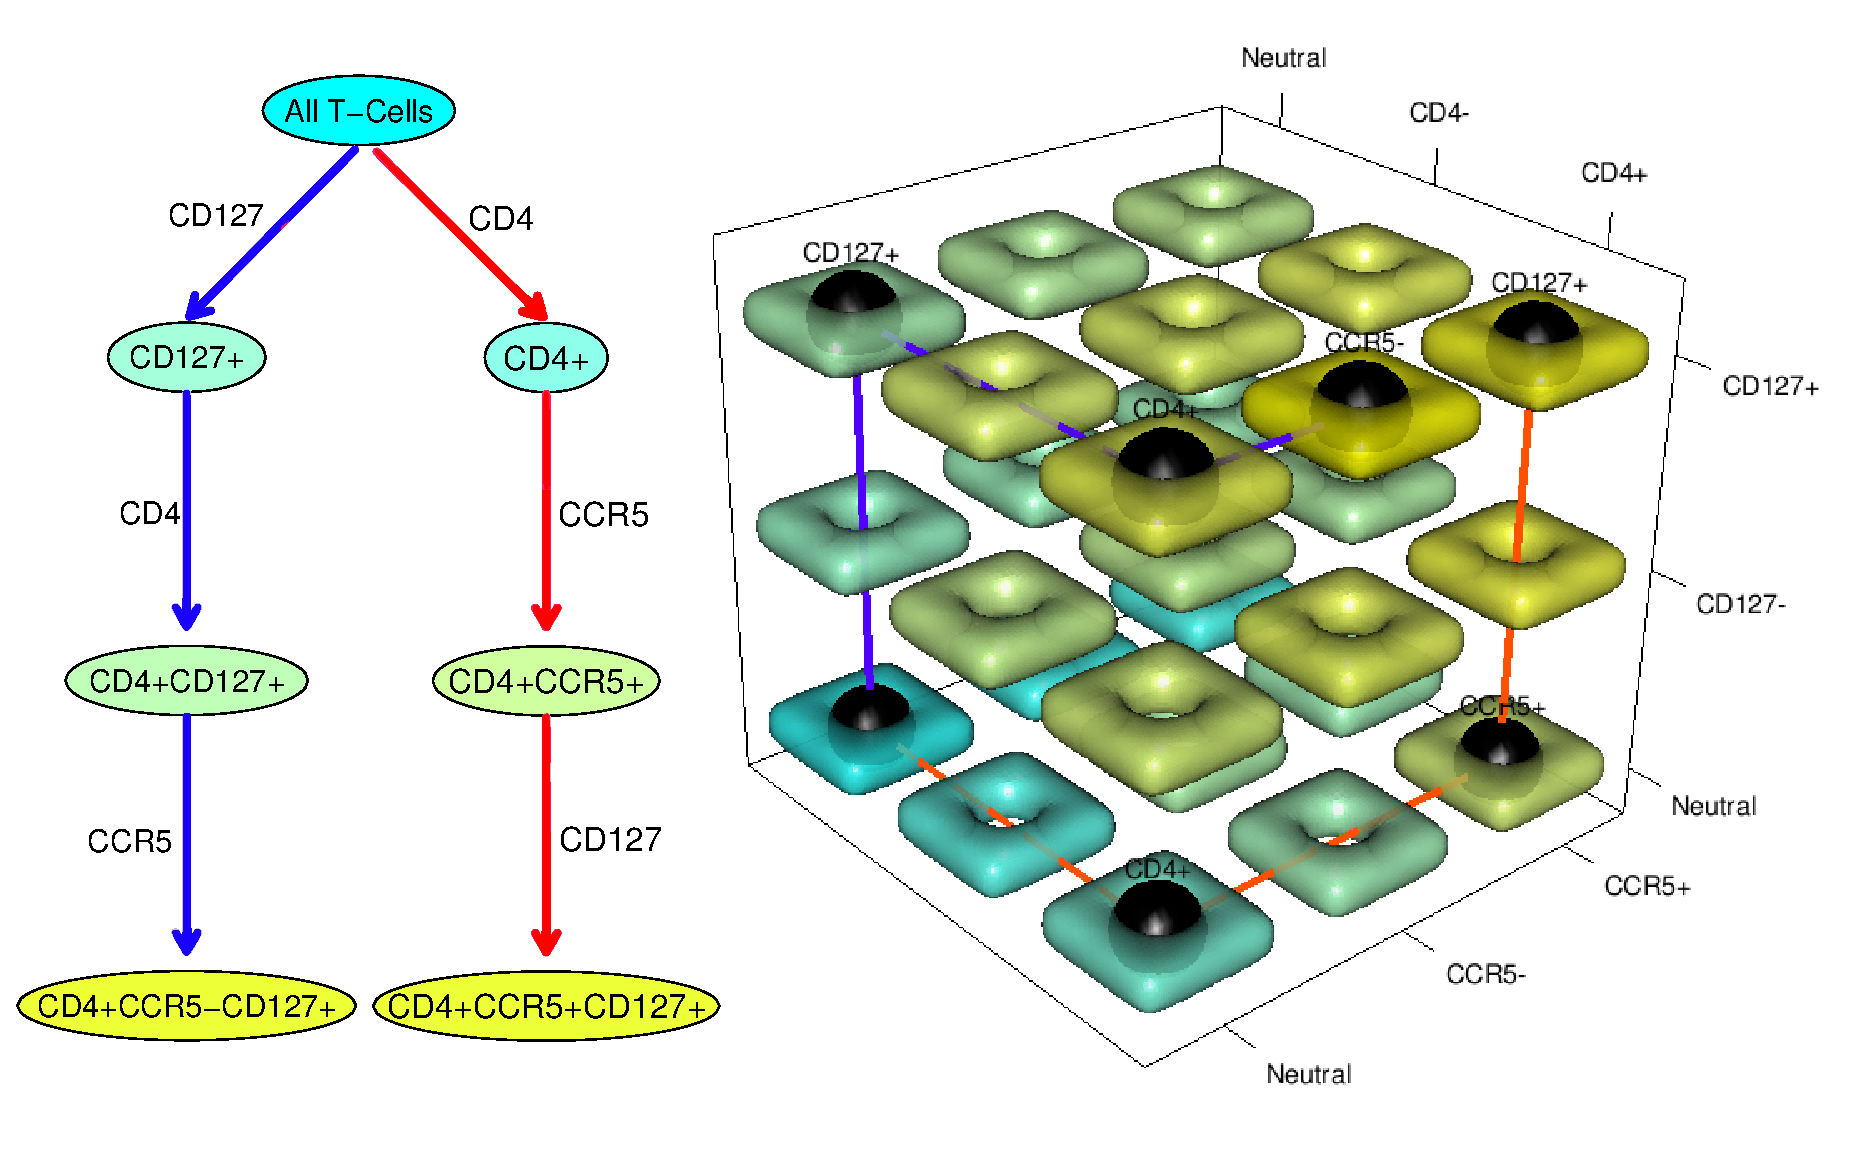
\includegraphics[width=15cm]{figs/rchy/2path}
  \end{center}
  \caption{Dynamic programming algorithm for two cell populations defined by $3$ markers.
    The best path for each of the cell population is shown in red and blue respectively.
    As an example, the red path ends at CD4$^+$CCR5$^+$CD127$^+$.
    Three markers are available to be added.
    First, CD4 is added (changes from does not matter to positive).
    Then two options will be available for the next step (CD127 and CCR5).
    After selection of CCR5, only one option will be left for the final step (CD127).
    Therefore for three markers, $\frac{3 \cdot (3-1)}{2}=6$ comparisons were required.
	\textbf{Left:} A hierarchy for the two paths. The label of an edge is the name of the single marker phenotype that
	is the difference between its head set ($s$) and its tail set ($t$).  \textbf{Right:} the dynamic programming space
	for the $3$ markers. Black spheres mark the nodes in the dynamic programing space used by the two paths. 
	The colors of the nodes on the left match that of the square tori on the right and  correspond to the relative score of each cell population. 
}
  \label{r1:3dDP}
\end{figure}
\end{landscape}

\begin{landscape}
\begin{figure}[!h]
  \begin{center}
    \begin{tabular}{c||c||c}
      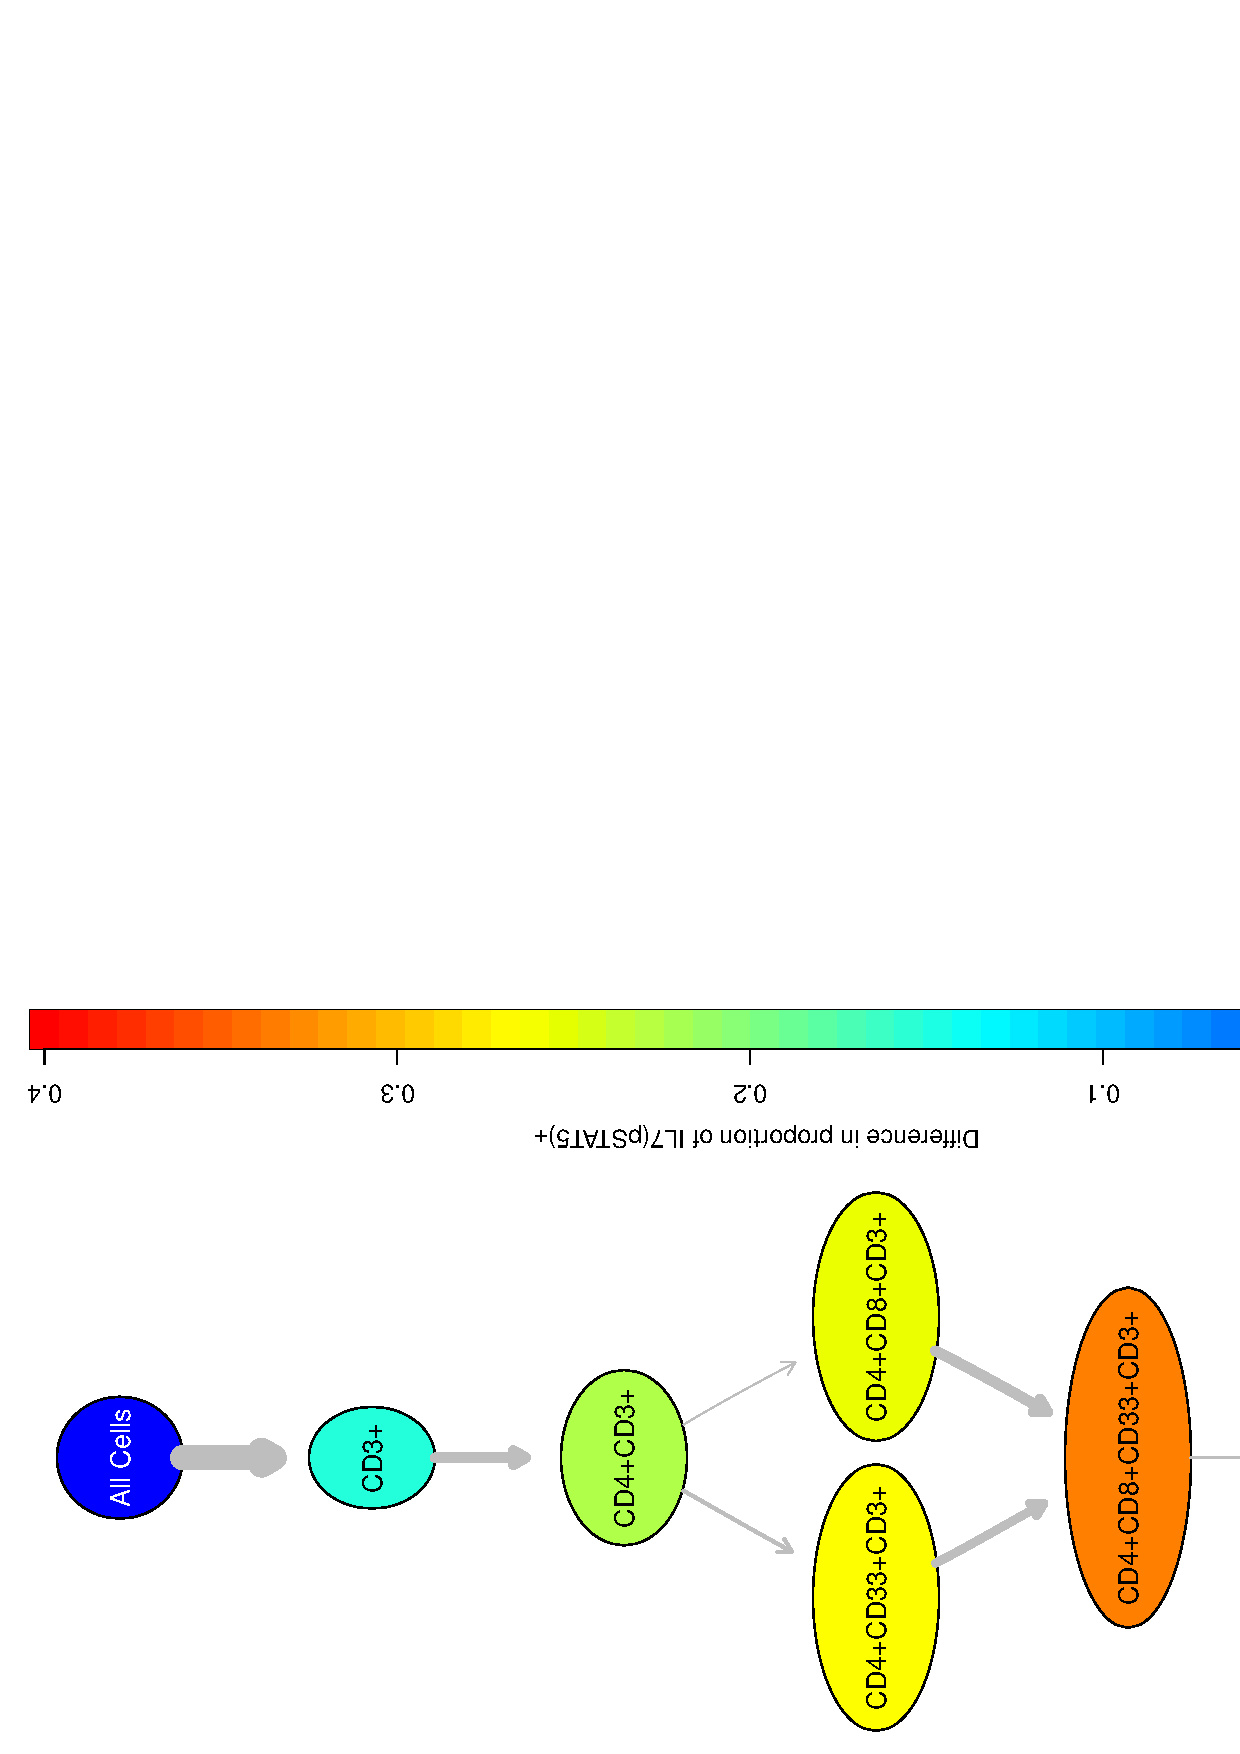
\includegraphics[width=4in,angle=270]{figs/rchy/IL7}&
      \includegraphics[width=4in,angle=270]{figs/rchy/BCR}&
      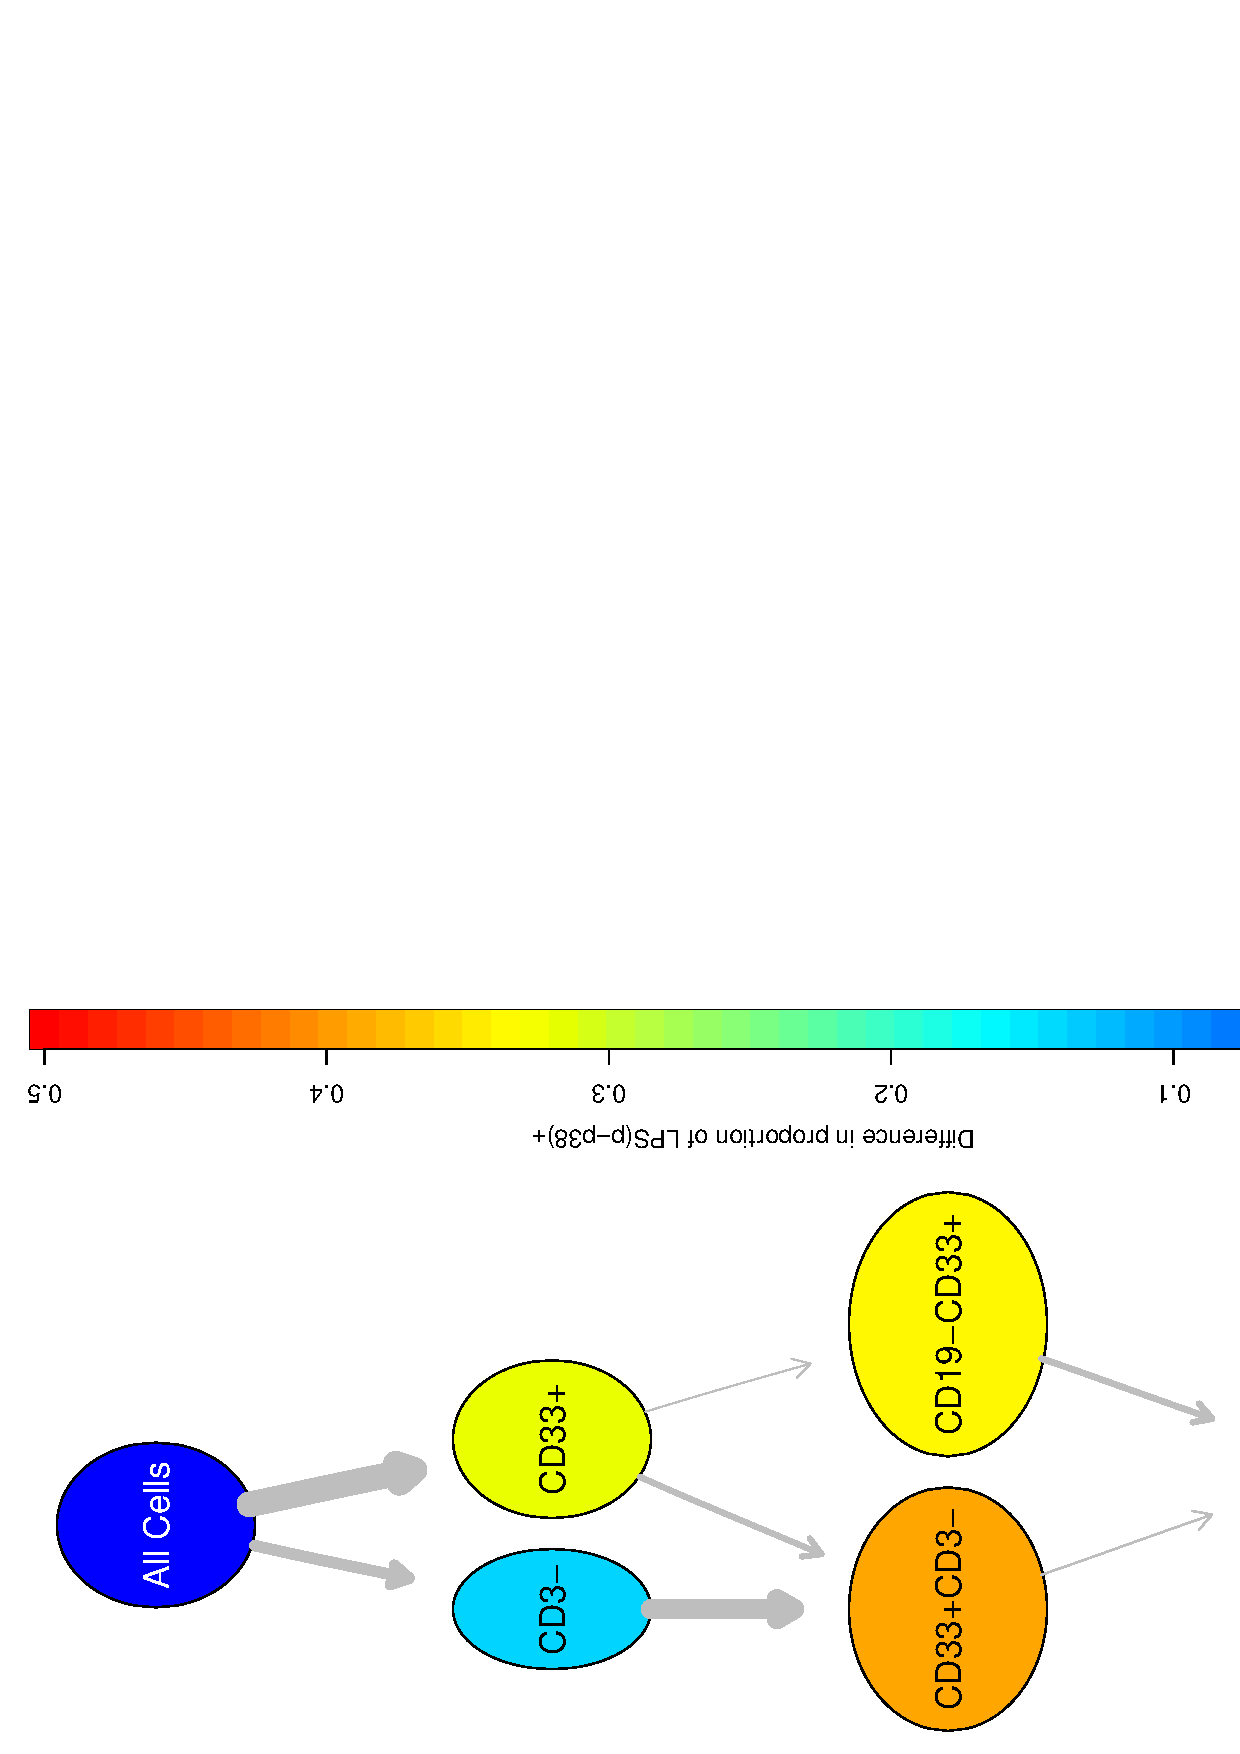
\includegraphics[width=4in,angle=270]{figs/rchy/LPS}\\
      (A) IL7/pSTAT5 &(B) BCR/pBLNK &(C) LPS/p-p38\\
    \end{tabular}
  \end{center}
  \caption{Three optimized hierarchies for identification of cell populations with maximum response to IL7, BCR, and LPS measured by pSTAT5, pBLNK, and p-p38, respectively.
    The colour of the nodes and the thickness of the edges shows the proportion and change in proportion of cells expressing the intracellular marker of interest, respectively.
  }
  \label{r1:CyTOF}
\end{figure}
\end{landscape}

\begin{figure}[ht]
  \begin{center}
    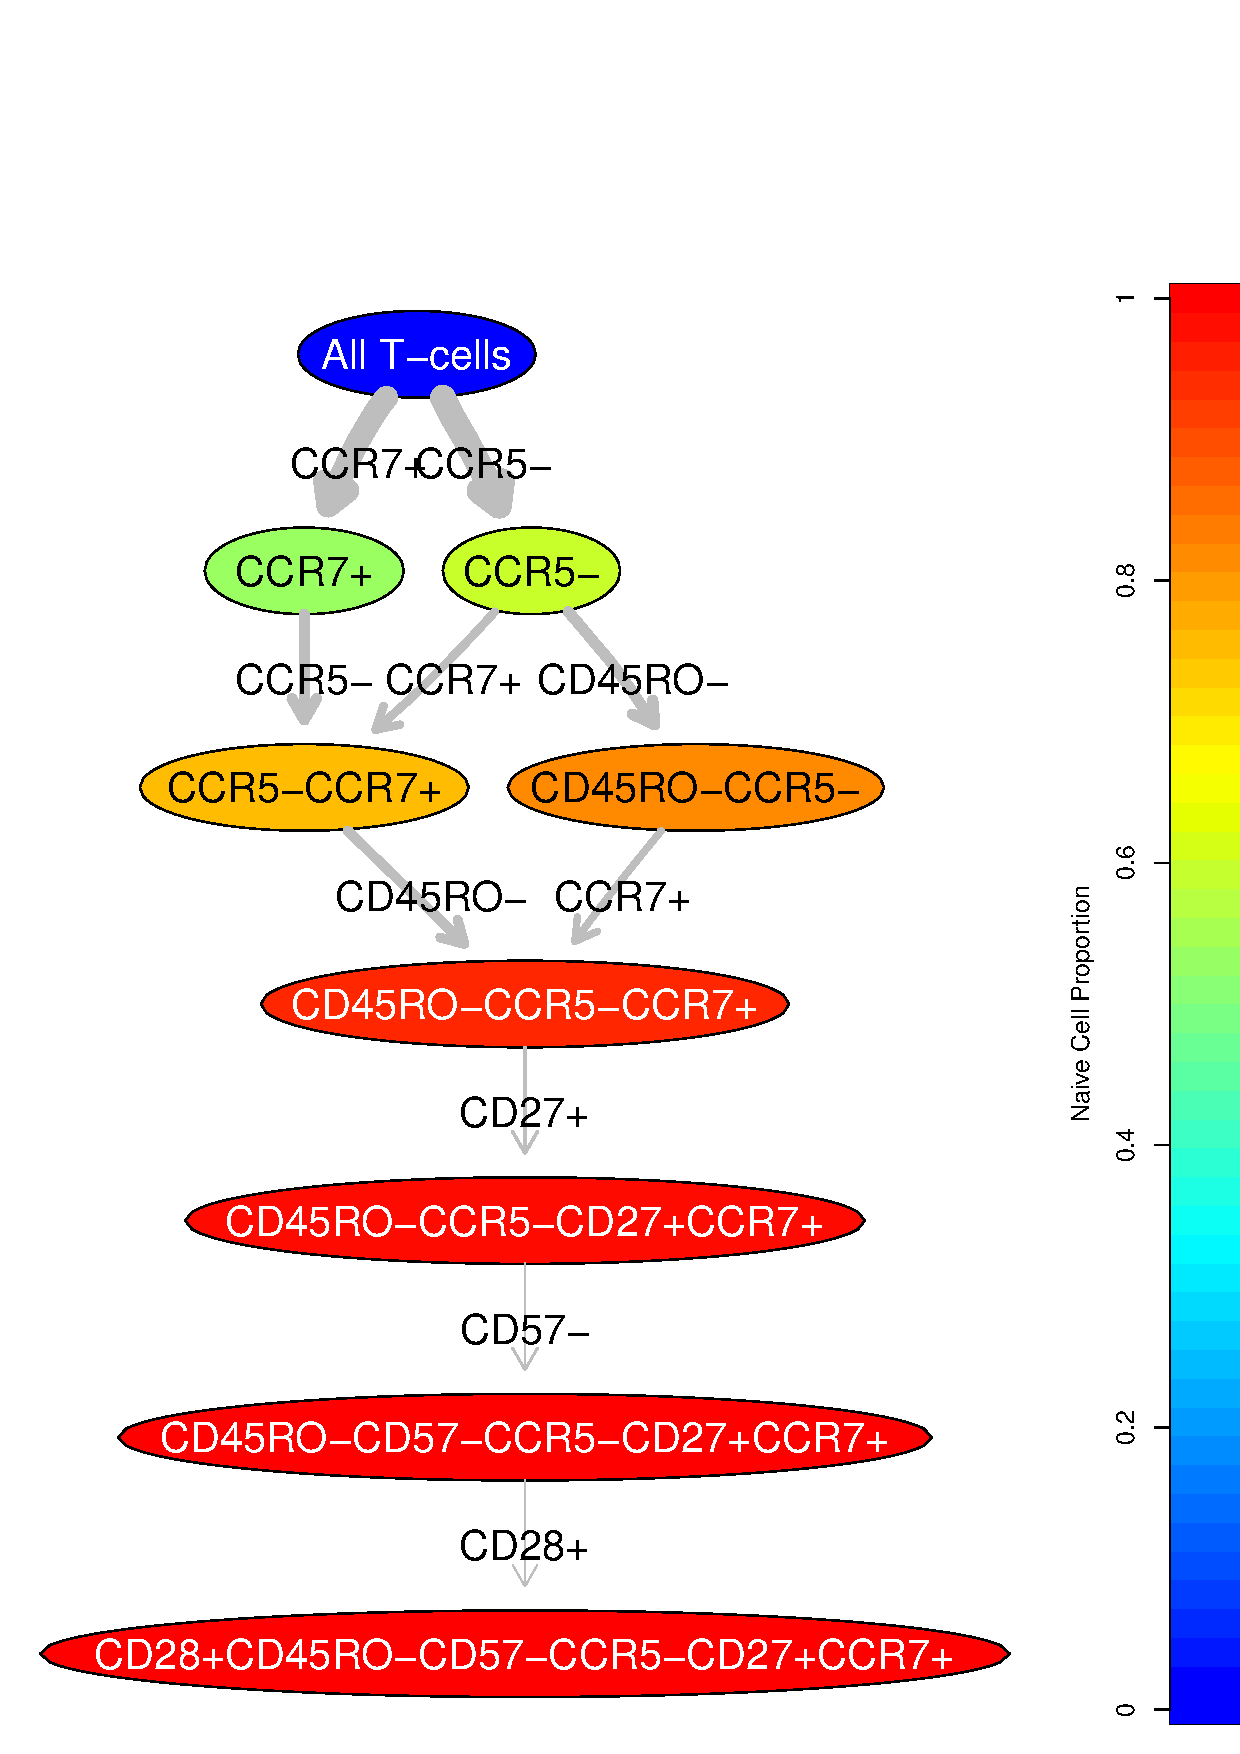
\includegraphics[width=4in]{figs/rchy/NaiveOverlap}
  \end{center}
  \caption{An optimized cellular hierarchy for identifying naive T-cells. The color of the nodes and the thickness of the edges shows the purity and change in purity of the original naive phenotype within the given cell population, respectively.
  }
  \label{r1:NaiveOverlap}
\end{figure}



\begin{landscape}
  \begin{figure}[ht]
    \begin{center}
      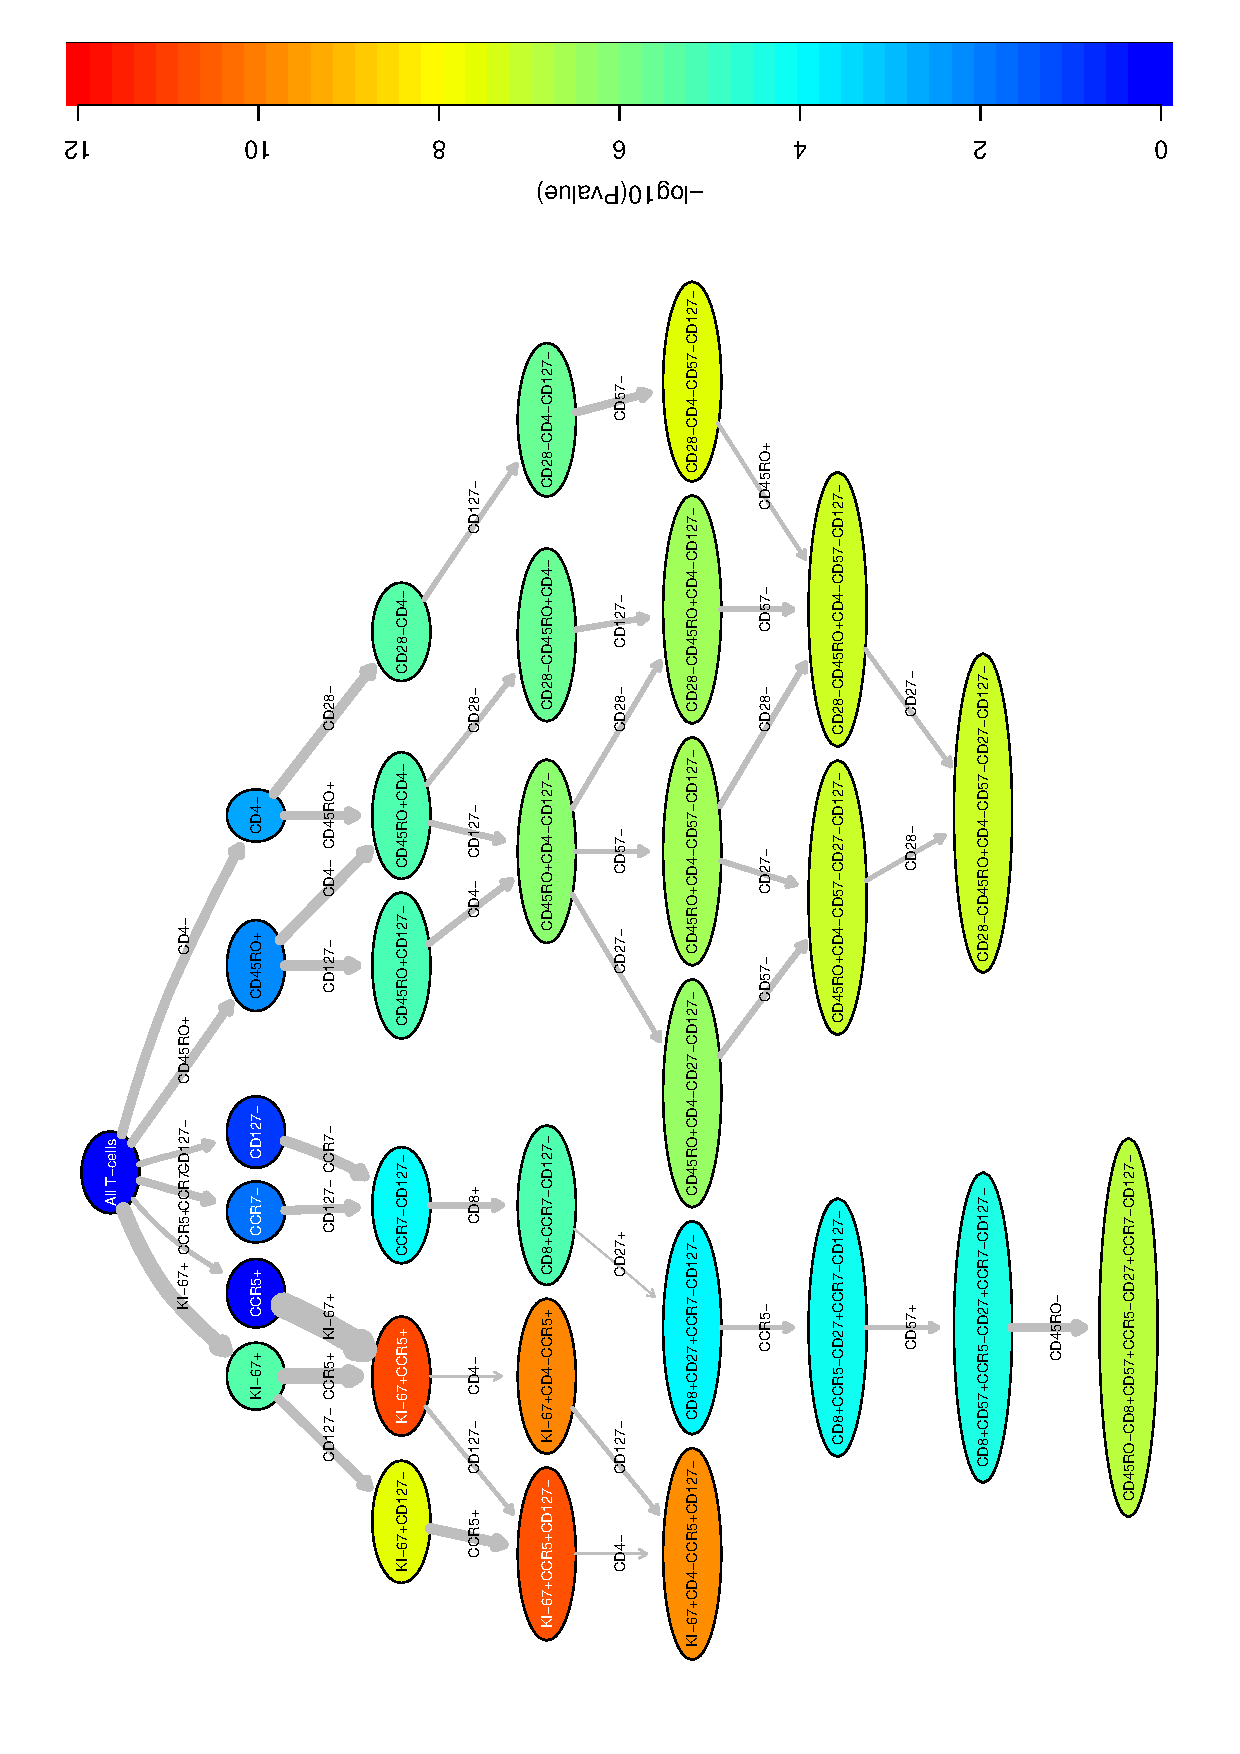
\includegraphics[width=\textwidth,angle=270]{figs/rchy/merged}
    \end{center}
    \caption{An optimized hierarchy for all three populations correlated with protection against HIV.
      The color of the nodes shows the significance of the correlation with the clinical outcome (p-value of the logrank test for the Cox proportional hazards model) and the width of each edge (arrow) shows the amount of change in this variable between the respective nodes.
      The positive and negative correlation of each immunophenotype with outcome can be seen from the arrow type leading to the node; however as all correlations are negative in this hierarchy, only one arrow type is shown. 
   }
    \label{r1:merged}
  \end{figure}
\end{landscape}



%\hide{
%  \begin{figure}[ht]
%    \begin{center}
%      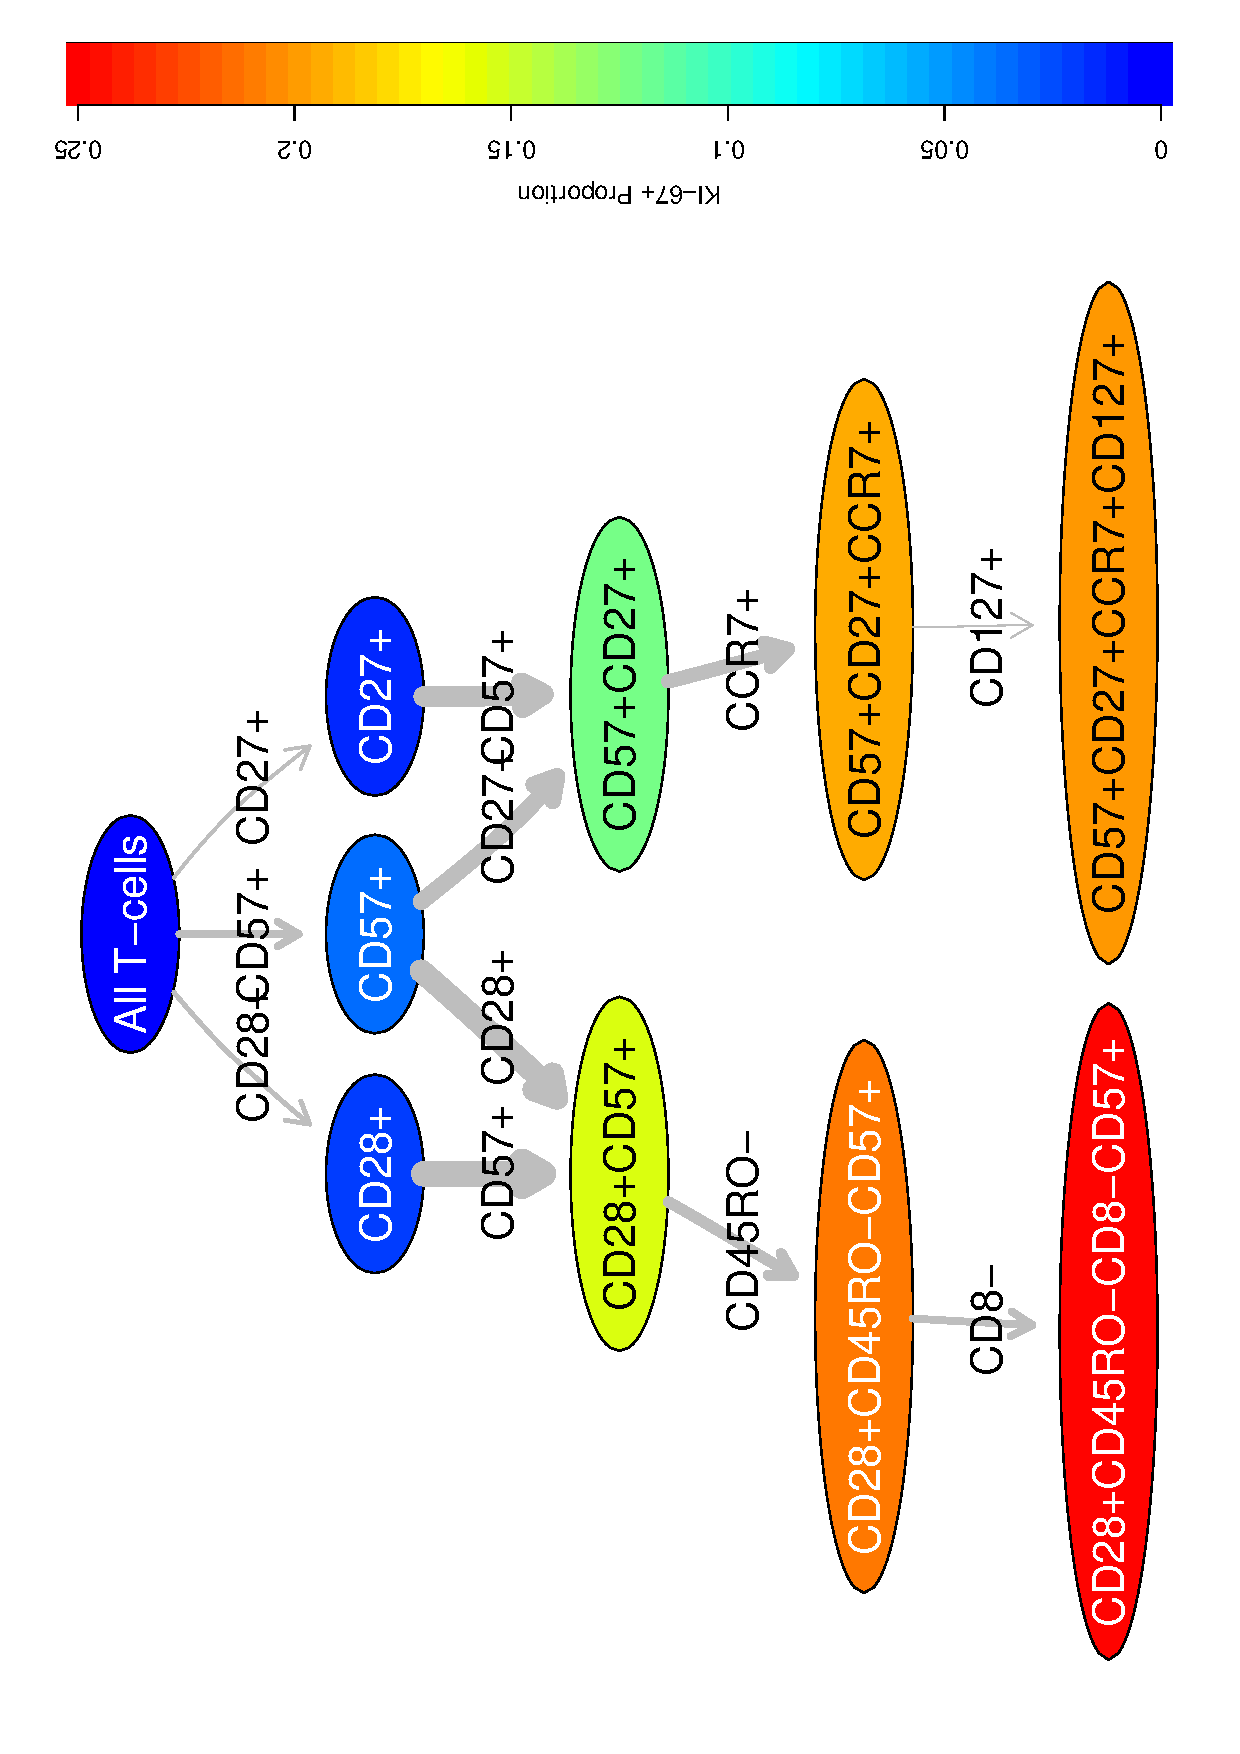
\includegraphics[width=13cm, angle=270]{figs/rchy/KI67Overlap}
%    \end{center}
%    \caption{A cellular hierarchy for identifying KI-67$^+$ T-cells using surface markers. The color of the nodes and the thickness of the edges shows the proportion and change in proportion of KI-67$^+$ T-cells, respectively.}
%    \label{r1:KI67Overlap}
%  \end{figure}
%}

\begin{table}[ht]\footnotesize
  \begin{center}
    \caption{The phenotypes with a high overlap with the BCR(pBLNK)$^+$ compartment as identified by flowType. The table includes the cell proportion of these immunophenotypes (second column) and the differences in the cell proportion of BCR(pBLNK)$^+$ cells in the stimulated and unstimulated assays (third column).}
    \label{BCR}
    \begin{tabular}{lll}
      \hline
      Phenotype Name & Cell Proportion & BCR$^+_{(stim-unstim)}$ \\ 
      \hline
      CD19+CD4-CD8-CD34+CD20+CD123+CD38-CD3- & 0.001 & 0.160 \\ 
      CD19+CD4-CD34+CD20+CD123+CD38-CD3- & 0.001 & 0.160 \\ 
      CD19+CD4-CD34+CD20+CD123+CD3- & 0.001 & 0.155 \\ 
      \hline
    \end{tabular}
  \end{center}
\end{table}


% latex table generated in R 2.14.1 by xtable 1.7-0 package
% Mon Mar 19 12:59:47 2012
\begin{table}[ht]\footnotesize
  \begin{center}
    \caption{The phenotypes with a high overlap with the IL7(pSTAT5)$^+$ compartment as identified by flowType. The table includes the cell proportion of these immunophenotypes (second column) and differences in the cell proportion of IL7(pSTAT5)$^+$ cells in the stimulated and unstimulated assays (third column).}
    \label{IL7}
    \begin{tabular}{lll}
      \hline
      Phenotype Name & Cell Proportion & IL7$^+_{(stim-unstim)}$ \\ 
      \hline
        CD19-CD4+CD8+CD20+CD33+CD38-CD3+ & 0.008 & 0.364 \\ 
        CD19-CD4+CD8+CD20+CD33+CD3+ & 0.008 & 0.366 \\ 
        CD19-CD4+CD8+CD34+CD33+CD38-CD3+ & 0.008 & 0.366 \\ 
        CD19-CD4+CD8+CD34+CD33+CD3+ & 0.008 & 0.368 \\ 
        CD19-CD4+CD8+CD34+CD20+CD33+CD38-CD3+ & 0.006 & 0.399 \\ 
        CD19-CD4+CD8+CD34+CD20+CD33+CD3+ & 0.006 & 0.402 \\ 
        CD4+CD8+CD20+CD33+CD38-CD3+ & 0.011 & 0.365 \\ 
        CD4+CD8+CD20+CD33+CD3+ & 0.011 & 0.371 \\ 
        CD4+CD8+CD34+CD33+CD38-CD3+ & 0.011 & 0.366 \\ 
        CD4+CD8+CD34+CD33+CD3+ & 0.011 & 0.371 \\ 
        CD4+CD8+CD34+CD20+CD33+CD38-CD3+ & 0.008 & 0.399 \\ 
        CD4+CD8+CD34+CD20+CD33+CD3+ & 0.009 & 0.405 \\ 
        CD19+CD4+CD8+CD20+CD33+CD38-CD3+ & 0.003 & 0.364 \\ 
        CD19+CD4+CD8+CD20+CD33+CD3+ & 0.003 & 0.378 \\ 
        CD19+CD4+CD8+CD34+CD33+CD38-CD3+ & 0.003 & 0.359 \\ 
        CD19+CD4+CD8+CD34+CD33+CD3+ & 0.003 & 0.372 \\ 
        CD19+CD4+CD8+CD34+CD20+CD33+CD38-CD3+ & 0.002 & 0.397 \\ 
        CD19+CD4+CD8+CD34+CD20+CD33+CD3+ & 0.002 & 0.409 \\ 
      \hline
    \end{tabular}
  \end{center}
\end{table}


% latex table generated in R 2.14.1 by xtable 1.7-0 package
% Mon Mar 19 12:55:05 2012
\begin{table}[ht]\footnotesize
  \begin{center}
    \caption{The phenotypes with a high overlap with the LPS(p-p38)$^+$ compartment as identified by flowType. The table includes the cell proportion of these immunophenotypes (second column) and differences in the cell proportion of LPS(p-p38)$^+$ cells in the stimulated and unstimulated assays (third column).}
    \label{LPS}
    \begin{tabular}{lll}
      \hline
      Phenotype Name & Cell Proportion & LPS$^+_{(stim-unstim)}$ \\ 
      \hline
      CD19-CD4-CD8-CD34-CD20-CD33+CD123-CD38-CD3- & 0.008 & 0.474 \\ 
      CD19-CD4-CD8-CD34-CD20-CD33+CD123-CD3- & 0.008 & 0.473 \\ 
      CD19-CD4-CD8-CD34-CD20-CD33+CD38-CD3- & 0.009 & 0.466 \\ 
      CD19-CD4-CD8-CD34-CD20-CD33+CD3- & 0.009 & 0.465 \\ 
      CD19-CD4-CD8-CD34-CD33+CD123-CD38-CD3- & 0.022 & 0.460 \\ 
      CD19-CD4-CD8-CD34-CD33+CD123-CD3- & 0.022 & 0.459 \\ 
      CD19-CD4-CD8-CD34-CD33+CD38-CD3- & 0.022 & 0.452 \\ 
      CD19-CD4-CD8-CD34-CD33+CD3- & 0.022 & 0.451 \\ 
      CD19-CD4-CD8-CD34-CD20+CD33+CD123-CD38-CD3- & 0.013 & 0.450 \\ 
      CD19-CD4-CD8-CD34-CD20+CD33+CD123-CD3- & 0.013 & 0.449 \\ 
      CD19-CD4-CD8-CD20-CD33+CD123-CD38-CD3- & 0.023 & 0.453 \\ 
      CD19-CD4-CD8-CD20-CD33+CD123-CD3- & 0.023 & 0.452 \\ 
      CD19-CD4-CD34-CD20-CD33+CD123-CD38-CD3- & 0.011 & 0.456 \\ 
      CD19-CD4-CD34-CD20-CD33+CD123-CD3- & 0.011 & 0.455 \\ 
      CD19-CD8-CD34-CD20-CD33+CD123-CD38-CD3- & 0.012 & 0.462 \\ 
      CD19-CD8-CD34-CD20-CD33+CD123-CD3- & 0.012 & 0.461 \\ 
      CD19-CD8-CD34-CD20-CD33+CD38-CD3- & 0.012 & 0.454 \\ 
      CD19-CD8-CD34-CD20-CD33+CD3- & 0.012 & 0.454 \\ 
      CD4-CD8-CD34-CD20-CD33+CD123-CD38-CD3- & 0.011 & 0.462 \\ 
      CD4-CD8-CD34-CD20-CD33+CD123-CD3- & 0.011 & 0.461 \\ 
      CD4-CD8-CD34-CD20-CD33+CD38-CD3- & 0.011 & 0.454 \\ 
      CD4-CD8-CD34-CD20-CD33+CD3- & 0.011 & 0.454 \\ 
      CD8-CD34-CD20-CD33+CD123-CD38-CD3- & 0.015 & 0.450 \\ 
      CD8-CD34-CD20-CD33+CD123-CD3- & 0.015 & 0.449 \\ 
      \hline
    \end{tabular}
  \end{center}
\end{table}

% latex table generated in R 2.11.1 by xtable 1.5-6 package
% Sat Dec 11 12:28:36 2010
% \begin{table}\tiny
\begin{landscape}
\begin{center}
  {\tiny 
    % \begin{longtable}{rp{6cm}lllll}
    \begin{longtable}{rlllllll}
      \caption{\normalsize Statistically significant immunophenotypic correlates of survival of HIV$^+$ subjects are predicted by flowType. The p-values of the log rank tests, 95\% confidence intervals calculated using bootstrapping, adjusted p-values using Bonferroni's method, coefficients and $R^2$ values of the Cox proportional hazards regression models, and the frequency of the cells are provided as columns of the table.}\\
 \hline
      \# & Phenotype & p-value & p-value, CI & adjusted & CPHR & R$^2$ & Cell \\
      &  & & & p-value & Coefficient &  & Frequency \\
      \hline
      \endhead
      1 & CD28-CD45RO+CD57-CCR5+ & 5.3e-07 & (4.3e-14, 1.3e-02) & 2e-02 &  20.5 & 0.056 & 0.03048 \\ 
      2 & CD28-CD8+CD57-CD127- & 2.5e-07 & (2.3e-14, 3.8e-04) & 1e-02 &  12.3 & 0.060 & 0.05975 \\ 
      3 & CD28-CD45RO+CD57-CCR7- & 5.1e-07 & (2.3e-14, 6.1e-04) & 2e-02 &  15.7 & 0.057 & 0.03829 \\ 
      4 & CD28-CD45RO+CD4-CD57- & 3.5e-07 & (2.3e-14, 1.1e-03) & 1e-02 &  13.2 & 0.058 & 0.04357 \\ 
      5 & CD45RO+CD4-CD57-CD127- & 2.7e-07 & (1.2e-13, 7.1e-03) & 1e-02 &  12.8 & 0.059 & 0.05062 \\ 
      6 & CD28-CD45RO+CD57-CD127- & 4.7e-08 & (1.7e-14, 6.8e-04) & 2e-03 &  16.0 & 0.067 & 0.03732 \\ 
      7 & CD45RO+CD4-CD27-CD127- & 4.4e-07 & (5.8e-14, 1.1e-03) & 2e-02 &  14.3 & 0.057 & 0.04830 \\ 
      8 & CD28-CD45RO+CD57- & 5.6e-07 & (4.4e-14, 4.1e-04) & 2e-02 &  12.4 & 0.056 & 0.05015 \\ 
      9 & CD45RO+CD4-CD127- & 6.5e-07 & (4.7e-15, 2.9e-03) & 2e-02 &   9.6 & 0.056 & 0.07176 \\ 
      10 & CD28-CD45RO+CD4-CD127- & 3.1e-07 & (0.0e+00, 5.7e-03) & 1e-02 &  11.7 & 0.059 & 0.05300 \\ 
      11 & CD28-CD45RO+CD57-CCR5+CD27-CCR7+CD127- & 4.7e-07 & (5.7e-14, 7.7e-03) & 2e-02 & 171.4 & 0.057 & 0.00315 \\ 
      12 & CD28-CD45RO+CD4-CD57-CCR5+CD27-CCR7+CD127- & 4.5e-07 & (1.8e-13, 3.9e-04) & 2e-02 & 176.2 & 0.057 & 0.00294 \\ 
      13 & CD28-CD57-CD127- & 3.3e-07 & (3.4e-15, 8.0e-03) & 1e-02 &   8.0 & 0.058 & 0.12341 \\ 
      14 & CD28-CD4-CD57- & 8.8e-07 & (2.2e-15, 2.9e-03) & 3e-02 &   7.2 & 0.054 & 0.15525 \\ 
      15 & CD57-CD27-CD127- & 6.2e-08 & (2.4e-14, 4.7e-03) & 2e-03 &   9.5 & 0.065 & 0.12173 \\ 
      16 & CD4-CD57-CD27-CD127- & 4.7e-08 & (4.2e-14, 3.3e-03) & 2e-03 &   9.7 & 0.067 & 0.09721 \\ 
      17 & CD28-CD57-CCR7-CD127- & 2.8e-07 & (9.7e-15, 1.0e-02) & 1e-02 &   9.8 & 0.059 & 0.08417 \\ 
      18 & CD28-CD4-CD57-CD127- & 3.3e-08 & (2.0e-12, 5.7e-04) & 1e-03 &   9.1 & 0.068 & 0.10852 \\ 
      19 & CD4-CD57-CCR7-CD127- & 6.5e-07 & (3.8e-15, 2.3e-03) & 2e-02 &   8.8 & 0.056 & 0.09501 \\ 
      20 & CD45RO-CD4-CD57+CCR5-CD27+CCR7-CD127- & 6.1e-07 & (1.2e-12, 2.6e-03) & 2e-02 & 498.4 & 0.056 & 0.00097 \\ 
      21 & CD28-CD45RO-CD4-CD57+CCR5-CD27+CCR7-CD127- & 2.5e-07 & (0.0e+00, 7.7e-03) & 1e-02 & 561.2 & 0.060 & 0.00074 \\ 
      22 & CD45RO-CD8+CD57+CCR5-CD27+CCR7-CD127- & 1.2e-07 & (4.6e-14, 3.3e-04) & 5e-03 & 638.6 & 0.063 & 0.00068 \\ 
      23 & CD45RO-CD8+CD4-CD57+CCR5-CD27+CCR7-CD127- & 1.2e-07 & (5.1e-14, 2.0e-03) & 5e-03 & 638.6 & 0.063 & 0.00068 \\ 
      24 & CD28-CD45RO-CD4-CD57+CCR5-CD27+CD127- & 5.7e-07 & (1.1e-13, 2.3e-03) & 2e-02 & 298.3 & 0.056 & 0.00099 \\ 
      25 & KI-67+CD28-CCR5+ & 1.0e-11 & (2.9e-13, 2.8e-03) & 4e-07 &  96.1 & 0.101 & 0.00547 \\ 
      26 & KI-67+CD28-CCR5+CD27- & 8.7e-12 & (1.5e-14, 8.9e-04) & 3e-07 & 115.3 & 0.102 & 0.00453 \\ 
      27 & KI-67+CCR5+ & 1.3e-11 & (2.4e-14, 7.0e-03) & 5e-07 &  53.4 & 0.100 & 0.01192 \\ 
      28 & KI-67+CD28+CD45RO+CD57-CCR7-CD127- & 4.2e-09 & (5.6e-16, 3.0e-03) & 2e-04 & 241.3 & 0.077 & 0.00209 \\ 
      29 & KI-67+CD45RO-CD4-CD27-CCR7-CD127- & 1.2e-09 & (2.0e-14, 4.4e-03) & 4e-05 & 161.9 & 0.082 & 0.00297 \\ 
      30 & KI-67+CD28-CD45RO-CD8-CD4- & 5.0e-09 & (2.9e-12, 1.7e-03) & 2e-04 & 176.0 & 0.076 & 0.00225 \\ 
      31 & KI-67+CD8-CD4- & 8.1e-09 & (6.1e-13, 4.5e-02) & 3e-04 &  58.1 & 0.074 & 0.00738 \\ 
      32 & KI-67+CCR5+CD27-CCR7- & 2.0e-11 & (3.8e-14, 6.0e-04) & 8e-07 & 109.8 & 0.099 & 0.00532 \\ 
      33 & KI-67+CD8-CCR5+CCR7- & 1.3e-10 & (3.1e-13, 2.0e-03) & 5e-06 & 147.3 & 0.091 & 0.00392 \\ 
      34 & KI-67+CD28-CD8-CCR5+CCR7+CD127- & 2.6e-09 & (1.6e-14, 1.1e-02) & 1e-04 & 625.8 & 0.079 & 0.00061 \\ 
      35 & KI-67+CD28+CD45RO+CD8+CD57-CD27+CCR7+ & 6.7e-07 & (3.8e-13, 1.5e-03) & 3e-02 & 585.4 & 0.055 & 0.00051 \\ 
      36 & KI-67+CD28+CD45RO+CD8+CD4-CD57-CD27+CCR7+ & 6.7e-07 & (1.1e-16, 4.7e-03) & 3e-02 & 585.4 & 0.055 & 0.00051 \\ 
      37 & KI-67+CD8+CD27-CCR7-CD127- & 4.7e-11 & (1.3e-13, 1.4e-03) & 2e-06 & 141.3 & 0.095 & 0.00292 \\ 
      38 & KI-67+CD8+CD4-CD27-CCR7-CD127- & 4.7e-11 & (1.3e-13, 1.3e-03) & 2e-06 & 141.3 & 0.095 & 0.00292 \\ 
      39 & KI-67+CD28-CD8+CD27-CCR7-CD127- & 2.7e-11 & (1.0e-13, 7.6e-04) & 1e-06 & 164.5 & 0.097 & 0.00241 \\ 
      40 & KI-67+CD28-CD8+CD4-CD27-CCR7-CD127- & 2.7e-11 & (2.7e-13, 1.4e-03) & 1e-06 & 164.5 & 0.097 & 0.00241 \\ 
      41 & KI-67+CD28-CD8+CCR7-CD127- & 6.6e-11 & (5.6e-14, 1.5e-02) & 3e-06 & 132.9 & 0.094 & 0.00293 \\ 
      42 & KI-67+CD28-CD8+CD4-CCR7-CD127- & 6.6e-11 & (1.2e-14, 8.4e-04) & 3e-06 & 132.9 & 0.094 & 0.00293 \\ 
      43 & KI-67+CD45RO+CD8+CD27-CCR7- & 1.2e-09 & (4.0e-12, 2.8e-03) & 5e-05 & 143.6 & 0.082 & 0.00216 \\ 
      44 & KI-67+CD45RO+CD8+CD4-CD27-CCR7- & 1.2e-09 & (1.0e-12, 1.2e-02) & 5e-05 & 143.6 & 0.082 & 0.00216 \\ 
      45 & KI-67+CD28-CD45RO+CD8+CD27-CCR7- & 1.0e-09 & (1.9e-15, 7.3e-04) & 4e-05 & 188.5 & 0.082 & 0.00155 \\ 
      46 & KI-67+CD28-CD45RO+CD8+CD4-CD27-CCR7- & 1.0e-09 & (1.7e-13, 2.0e-03) & 4e-05 & 188.5 & 0.082 & 0.00155 \\ 
      47 & KI-67+CD45RO+CD8+CD27-CD127- & 7.1e-10 & (1.2e-14, 6.8e-03) & 3e-05 & 152.4 & 0.084 & 0.00221 \\ 
      48 & KI-67+CD45RO+CD8+CD4-CD27-CD127- & 7.1e-10 & (3.4e-14, 1.5e-03) & 3e-05 & 152.4 & 0.084 & 0.00221 \\ 
      49 & KI-67+CD28-CD45RO+CD8+CD27-CD127- & 5.0e-10 & (6.0e-13, 3.1e-03) & 2e-05 & 201.3 & 0.085 & 0.00163 \\ 
      50 & KI-67+CD28-CD45RO+CD8+CD4-CD27-CD127- & 5.0e-10 & (4.6e-14, 2.7e-03) & 2e-05 & 201.3 & 0.085 & 0.00163 \\ 
      51 & KI-67+CD28-CD45RO+CD8+CD127- & 1.0e-09 & (1.2e-15, 3.2e-03) & 4e-05 & 150.5 & 0.083 & 0.00222 \\ 
      52 & KI-67+CD28-CD45RO+CD8+CD4-CD127- & 1.0e-09 & (1.5e-11, 3.6e-03) & 4e-05 & 150.5 & 0.083 & 0.00222 \\ 
      53 & KI-67+CD45RO+CD8+CD4-CD127- & 2.2e-09 & (2.8e-13, 2.1e-03) & 9e-05 &  99.8 & 0.079 & 0.00362 \\ 
      54 & KI-67+CD28-CD45RO+CD8+CD4-CCR7- & 8.0e-09 & (2.7e-12, 7.2e-04) & 3e-04 & 133.6 & 0.074 & 0.00209 \\ 
      55 & KI-67+CD28-CD45RO+CD57-CCR7+CD127- & 5.9e-08 & (4.0e-15, 4.5e-03) & 2e-03 & 376.6 & 0.066 & 0.00075 \\ 
      56 & KI-67+CD28-CD45RO+CD4-CD57-CCR7+CD127- & 5.0e-08 & (4.8e-13, 3.9e-03) & 2e-03 & 409.6 & 0.066 & 0.00070 \\ 
      57 & KI-67+CD57-CD27-CD127- & 5.9e-10 & (3.2e-14, 2.7e-03) & 2e-05 &  44.9 & 0.085 & 0.00806 \\ 
      58 & KI-67+CD28-CD27-CD127- & 4.8e-10 & (7.3e-15, 2.5e-03) & 2e-05 &  50.6 & 0.086 & 0.00711 \\ 
      59 & KI-67+CD4-CD127- & 1.3e-10 & (4.4e-16, 9.7e-03) & 5e-06 &  37.1 & 0.091 & 0.01159 \\ 
      60 & KI-67+CD28-CD127- & 4.9e-10 & (1.1e-12, 1.4e-03) & 2e-05 &  41.4 & 0.086 & 0.00823 \\ 
      61 & KI-67+CD4-CD27- & 5.6e-09 & (2.1e-14, 2.6e-03) & 2e-04 &  28.6 & 0.075 & 0.01122 \\ 
      62 & KI-67+CD28-CD4-CD27- & 1.8e-09 & (3.6e-13, 5.3e-03) & 7e-05 &  40.2 & 0.080 & 0.00785 \\ 
      63 & KI-67+CD27-CD127- & 1.3e-09 & (9.8e-15, 1.1e-03) & 5e-05 &  33.0 & 0.082 & 0.01052 \\ 
      64 & KI-67+CCR7-CD127- & 6.5e-11 & (1.4e-15, 9.6e-04) & 2e-06 &  47.3 & 0.094 & 0.00947 \\ 
      65 & KI-67+CD4-CD27-CCR7- & 9.6e-11 & (1.1e-16, 1.5e-03) & 4e-06 &  52.1 & 0.092 & 0.00764 \\ 
      66 & KI-67+CD4-CCR7- & 1.7e-10 & (3.0e-14, 1.0e-02) & 7e-06 &  41.4 & 0.090 & 0.00987 \\ 
      67 & KI-67+CD45RO+CD57-CCR7- & 1.4e-09 & (6.6e-13, 1.2e-03) & 5e-05 &  49.6 & 0.081 & 0.00695 \\ 
      68 & KI-67+CD45RO+CD57-CD27-CCR7- & 9.1e-10 & (8.6e-12, 2.5e-03) & 3e-05 &  66.4 & 0.083 & 0.00505 \\ 
      69 & KI-67+CD45RO+CD4- & 2.0e-09 & (8.0e-13, 2.5e-03) & 8e-05 &  45.3 & 0.080 & 0.00851 \\ 
      70 & KI-67+CD28-CD45RO+ & 1.3e-08 & (1.2e-12, 2.4e-03) & 5e-04 &  54.9 & 0.072 & 0.00525 \\ 
      71 & KI-67+CD45RO+CD127- & 1.1e-09 & (4.4e-16, 1.5e-02) & 4e-05 &  42.5 & 0.082 & 0.00834 \\ 
      72 & KI-67+CD45RO+CD57-CD127- & 2.9e-10 & (1.5e-14, 6.4e-04) & 1e-05 &  55.0 & 0.088 & 0.00719 \\ 
      73 & KI-67+CD28-CD45RO+CD8+CD27- & 9.2e-09 & (2.6e-15, 2.3e-03) & 4e-04 & 138.0 & 0.073 & 0.00201 \\ 
      74 & KI-67+CD28-CD45RO+CD8+CD4-CD27- & 9.2e-09 & (1.0e-15, 4.6e-03) & 4e-04 & 138.0 & 0.073 & 0.00201 \\ 
      75 & KI-67+CD8+CD4-CD57-CD27-CD127- & 1.9e-09 & (5.9e-14, 7.0e-03) & 7e-05 & 113.8 & 0.080 & 0.00274 \\ 
      76 & KI-67+CD28-CD45RO+CD8+ & 9.3e-09 & (5.9e-13, 1.4e-03) & 4e-04 & 102.7 & 0.073 & 0.00279 \\ 
      77 & KI-67+CD28-CD45RO+CD8+CD4- & 9.3e-09 & (0.0e+00, 1.6e-03) & 4e-04 & 102.7 & 0.073 & 0.00279 \\ 
      78 & KI-67+CD45RO+CD8+ & 2.1e-08 & (6.9e-15, 6.8e-04) & 8e-04 &  59.1 & 0.070 & 0.00512 \\ 
      79 & KI-67+CD8+CCR7- & 3.0e-08 & (7.7e-13, 2.8e-03) & 1e-03 &  49.5 & 0.068 & 0.00530 \\ 
      80 & KI-67+CD8+CD27-CCR7- & 8.3e-09 & (1.0e-13, 3.6e-03) & 3e-04 &  70.7 & 0.074 & 0.00377 \\ 
      81 & KI-67+CD4- & 2.8e-08 & (1.0e-13, 2.3e-03) & 1e-03 &  17.1 & 0.069 & 0.01627 \\ 
      82 & KI-67+CD28-CD4- & 1.1e-08 & (5.9e-14, 4.0e-03) & 4e-04 &  26.7 & 0.073 & 0.00950 \\ 
      83 & KI-67+CD127- & 2.7e-08 & (1.2e-12, 2.1e-03) & 1e-03 &  19.1 & 0.069 & 0.01460 \\ 
      84 & KI-67+CCR7- & 8.4e-08 & (3.4e-15, 2.3e-03) & 3e-03 &  18.3 & 0.064 & 0.01311 \\ 
      85 & KI-67+CD27-CCR7- & 3.5e-08 & (1.7e-13, 1.2e-03) & 1e-03 &  25.2 & 0.068 & 0.00998 \\ 
      86 & KI-67+CD45RO+CD27- & 7.5e-07 & (5.4e-13, 1.8e-03) & 3e-02 &  24.0 & 0.055 & 0.00862 \\ 
      87 & KI-67+CD45RO+CD57- & 1.2e-07 & (2.1e-13, 3.1e-03) & 5e-03 &  22.9 & 0.062 & 0.01123 \\ 
      88 & KI-67+CD4-CD57- & 1.3e-08 & (3.8e-15, 2.1e-03) & 5e-04 &  25.3 & 0.072 & 0.01209 \\ 
      89 & KI-67+CD28-CD4-CD57- & 9.7e-09 & (5.5e-12, 1.2e-03) & 4e-04 &  37.7 & 0.073 & 0.00698 \\ 
      90 & KI-67+CD57-CD127- & 3.3e-09 & (1.3e-13, 3.3e-03) & 1e-04 &  28.1 & 0.078 & 0.01128 \\ 
      91 & KI-67+CD45RO+CCR7- & 4.2e-09 & (7.8e-15, 2.5e-03) & 2e-04 &  37.5 & 0.077 & 0.00819 \\ 
      92 & KI-67+CD57-CCR7- & 2.7e-08 & (2.8e-13, 2.8e-03) & 1e-03 &  26.6 & 0.069 & 0.01008 \\ 
      93 & KI-67+CD57-CD27-CCR7- & 1.2e-08 & (4.9e-13, 2.6e-03) & 5e-04 &  36.8 & 0.072 & 0.00762 \\ 
      94 & KI-67+CD28-CCR7- & 3.3e-09 & (4.6e-14, 5.7e-03) & 1e-04 &  37.7 & 0.078 & 0.00739 \\ 
      95 & KI-67+CD28-CD27-CCR7- & 3.3e-09 & (2.6e-14, 6.5e-04) & 1e-04 &  43.0 & 0.078 & 0.00647 \\ 
      96 & KI-67+CD28- & 1.9e-07 & (4.0e-15, 2.7e-03) & 7e-03 &  18.3 & 0.061 & 0.01053 \\ 
      97 & KI-67+CD28-CD27- & 7.1e-08 & (1.5e-12, 8.6e-04) & 3e-03 &  26.3 & 0.065 & 0.00874 \\ 
      98 & KI-67+CD28-CD8- & 8.3e-08 & (5.5e-14, 2.5e-03) & 3e-03 &  44.2 & 0.064 & 0.00523 \\ 
      99 & KI-67+CD45RO+ & 8.9e-07 & (1.9e-13, 2.5e-03) & 3e-02 &  15.4 & 0.054 & 0.01343 \\ 
      100 & KI-67+CD8+CD57- & 1.1e-06 & (4.4e-14, 3.1e-03) & 4e-02 &  28.3 & 0.053 & 0.00648 \\ 
      101 & KI-67+CD8+CD27- & 6.4e-07 & (2.3e-14, 1.1e-02) & 2e-02 &  35.2 & 0.056 & 0.00560 \\ 
      \hline
      \label{ts1}
      % \end{table}
    \end{longtable}
  }
\end{center}
\end{landscape}

  \begin{landscape}
    \begin{figure}[ht]
      \begin{center}
        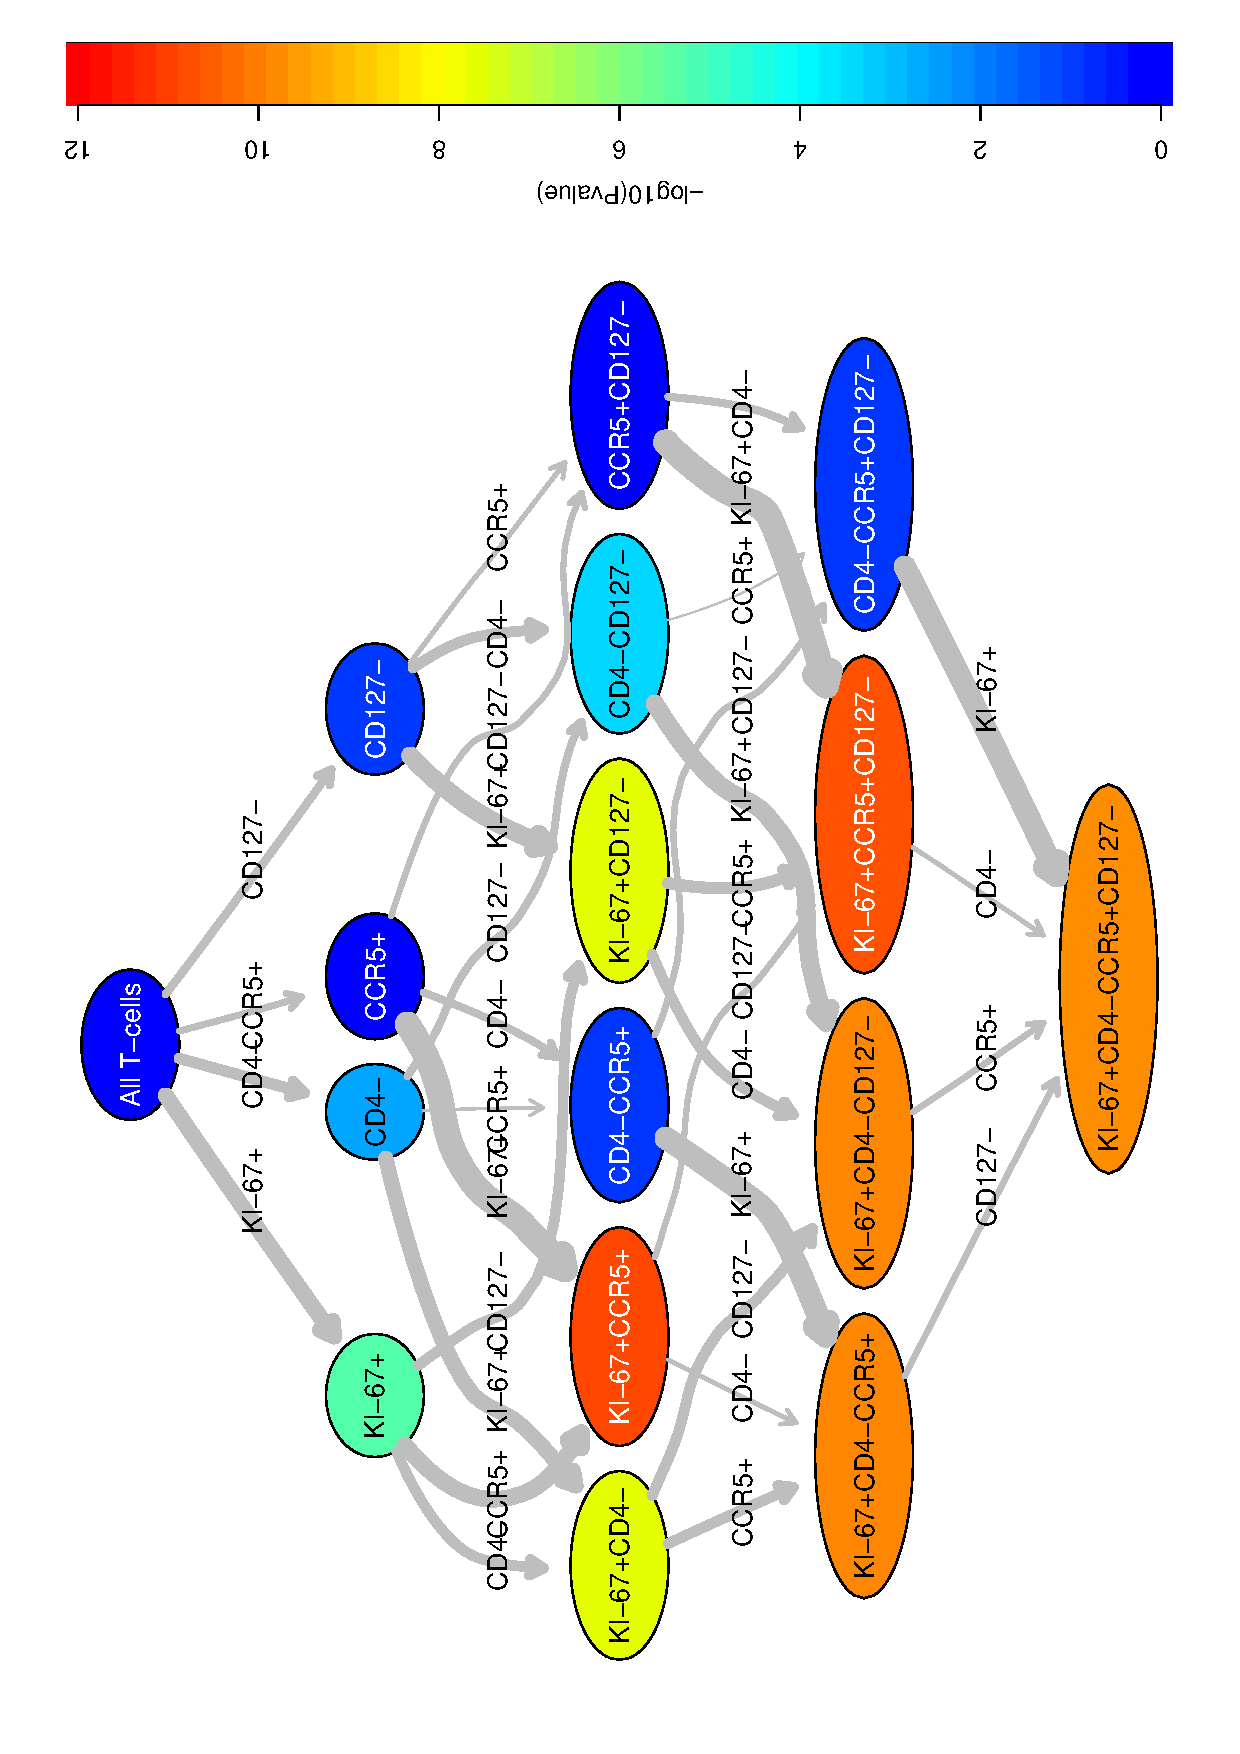
\includegraphics[width=13cm, angle=270]{figs/rchy/figs/HIVClinicalOutcomeComplete}
      \end{center}
      \caption{A complete cellular hierarchy for prediction of HIV's clinical outcome using KI67$^+$CD4$^-$CCR5$^+$CD127$^-$ T-cells. 
      The color of the nodes indicates the significance of the correlation with clinical outcome (p-value of the logrank test for the Cox proportional hazards model) and the width of each edge (arrow) shows the amount of change in this variable between the respective nodes.
        The positive and negative correlation of each immunophenotype with outcome can be seen from the arrow type leading to the node; however, as all correlations are negative in this hierarchy, only one arrow type is shown. 
      }
      \label{r1:HIVClinicalOutcomeComplete}
    \end{figure}
  \end{landscape}

  \begin{figure}[ht]
    \begin{center}
      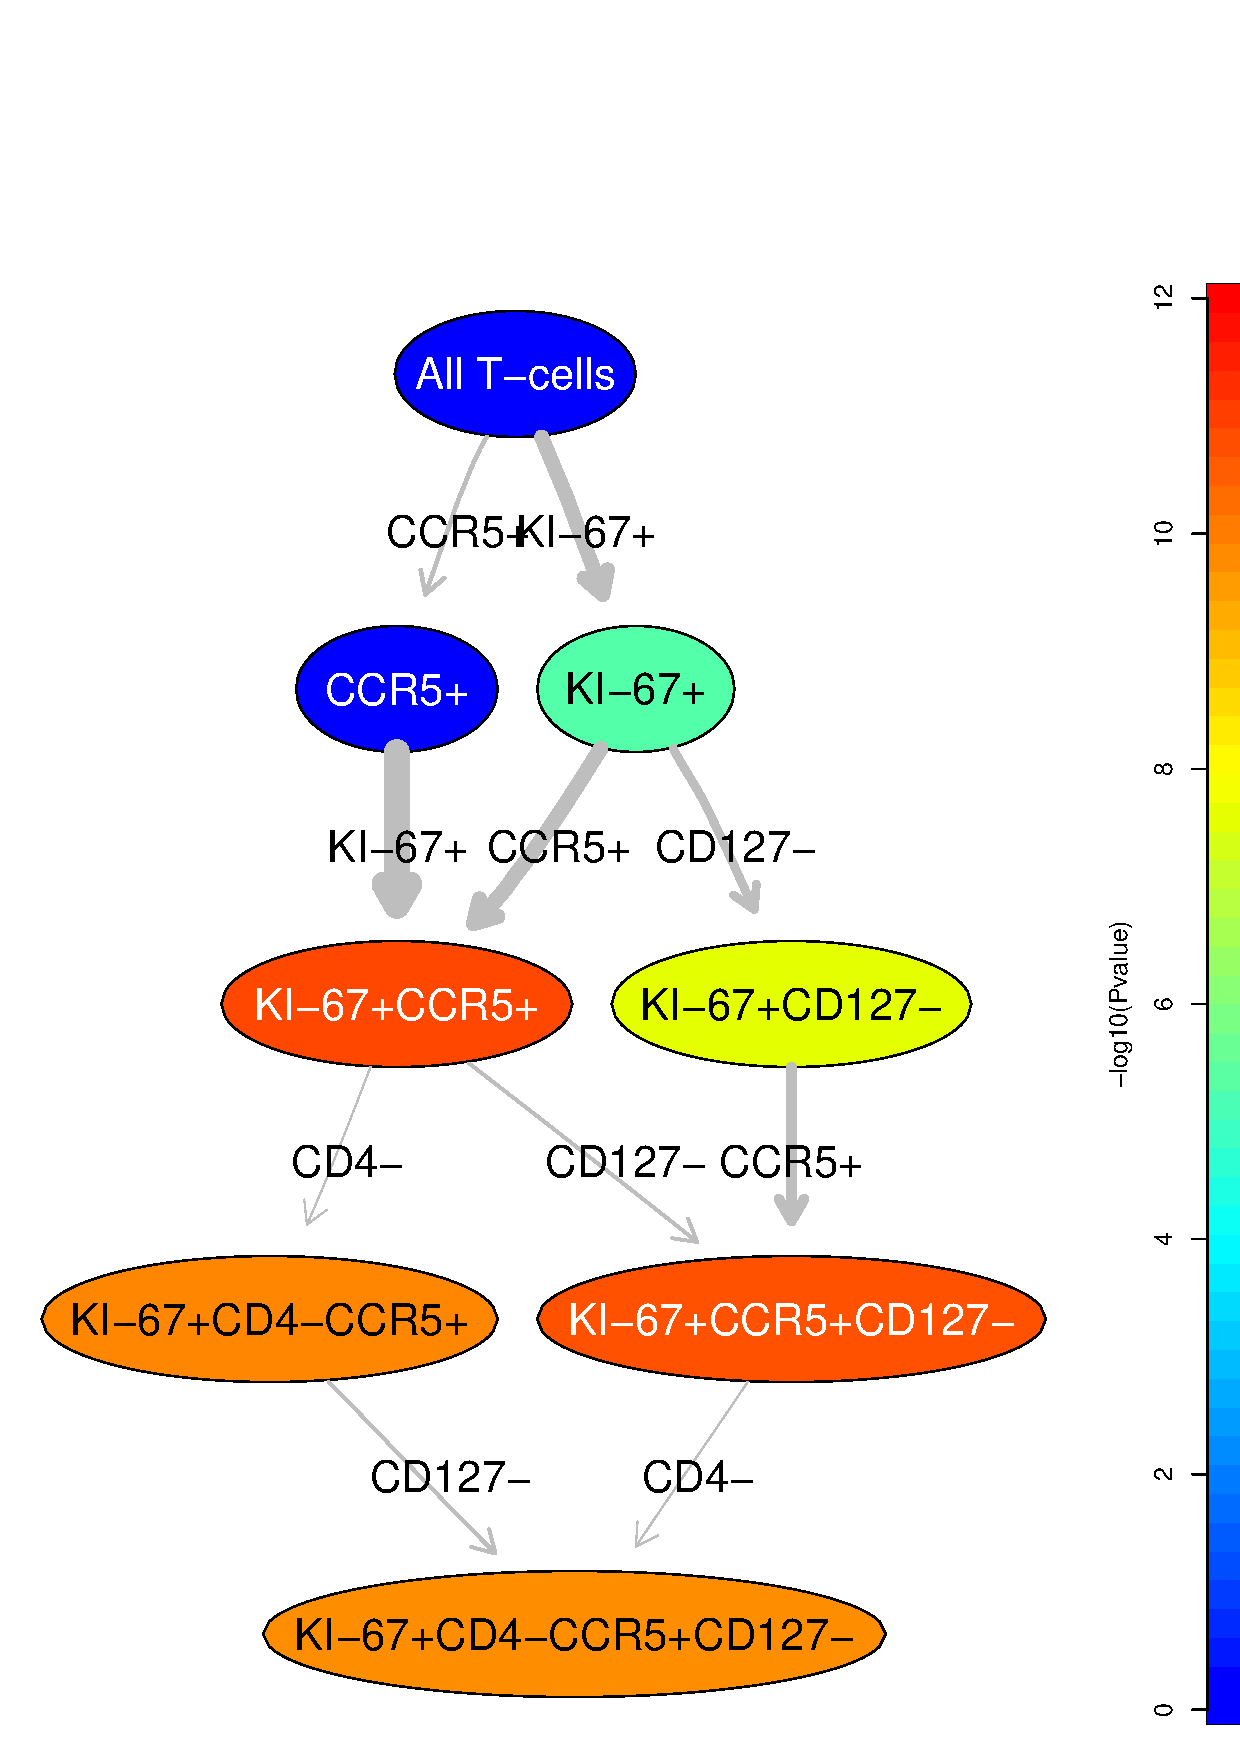
\includegraphics[width=13cm]{figs/rchy/figs/HIVClinicalOutcome}
    \end{center}
    \caption{An optimized cellular hierarchy for prediction of HIV's clinical outcome using KI67$^+$CD4$^-$CCR5$^+$CD127$^-$ T-cells. 
The color of the nodes shows the significance of the correlation with clinical outcome (p-value of the logrank test for the Cox proportional hazards model) and the width of each edge (arrow) shows the amount of change in this variable between the respective nodes. 
}
    \label{r1:HIVClinicalOutcome}
  \end{figure}

\begin{landscape}
\begin{figure}[!ht]
  \begin{center}
    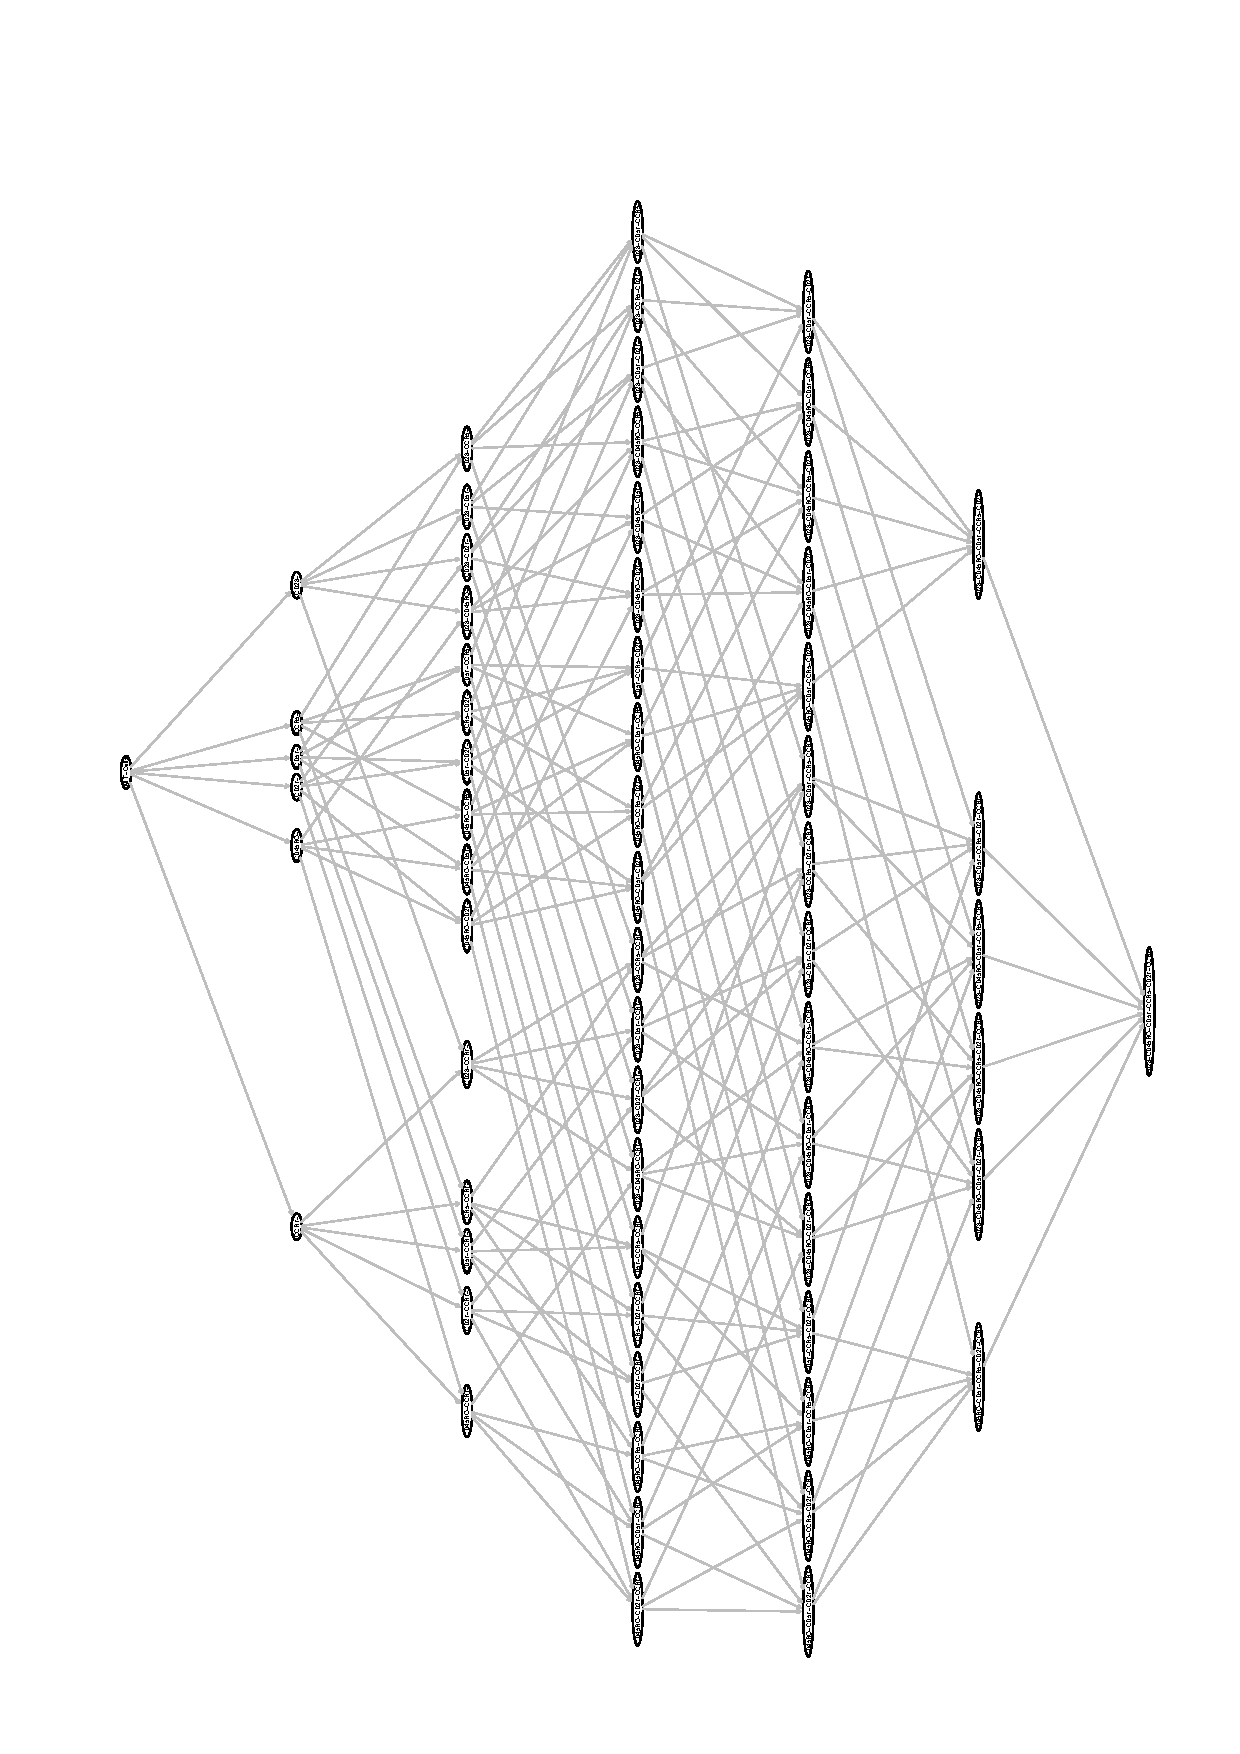
\includegraphics[width=13cm, angle=270]{figs/rchy/figs/NaiveOverlapComplete}
  \end{center}
  \caption{A complete cellular hierarchy for identifying naive T-cells. The colour of the nodes and the thickness of the edges have been removed to facilitate visualization of the complex graph.
  }
  \label{r1:NaiveOverlapComplete}
\end{figure}
\end{landscape}

  \begin{figure}[ht]
    \begin{center}
      \includegraphics[height=9cm, angle=0]{figs/rchy/figs/cdf}
    \end{center}
    \caption{Empirical cumulative distribution function of the $24$ possible paths (one dot per path, with some dots overlapping) for constructing the KI67$^+$CD4$^-$CCR5$^+$CD127$^-$ population. A change point in the path scores was defined manually (the red dashed line). The paths above the dashed line are those selected for construction of Figure \ref{r1:HIVClinicalOutcome}.}
    \label{r1:cdf}
  \end{figure}


  \begin{landscape}
  \begin{figure}[!ht]
    \begin{center}
      \begin{tabular}{c||c||c}
        \includegraphics[width=4in,angle=270]{figs/rchy/figs/IL7Proportions}&
        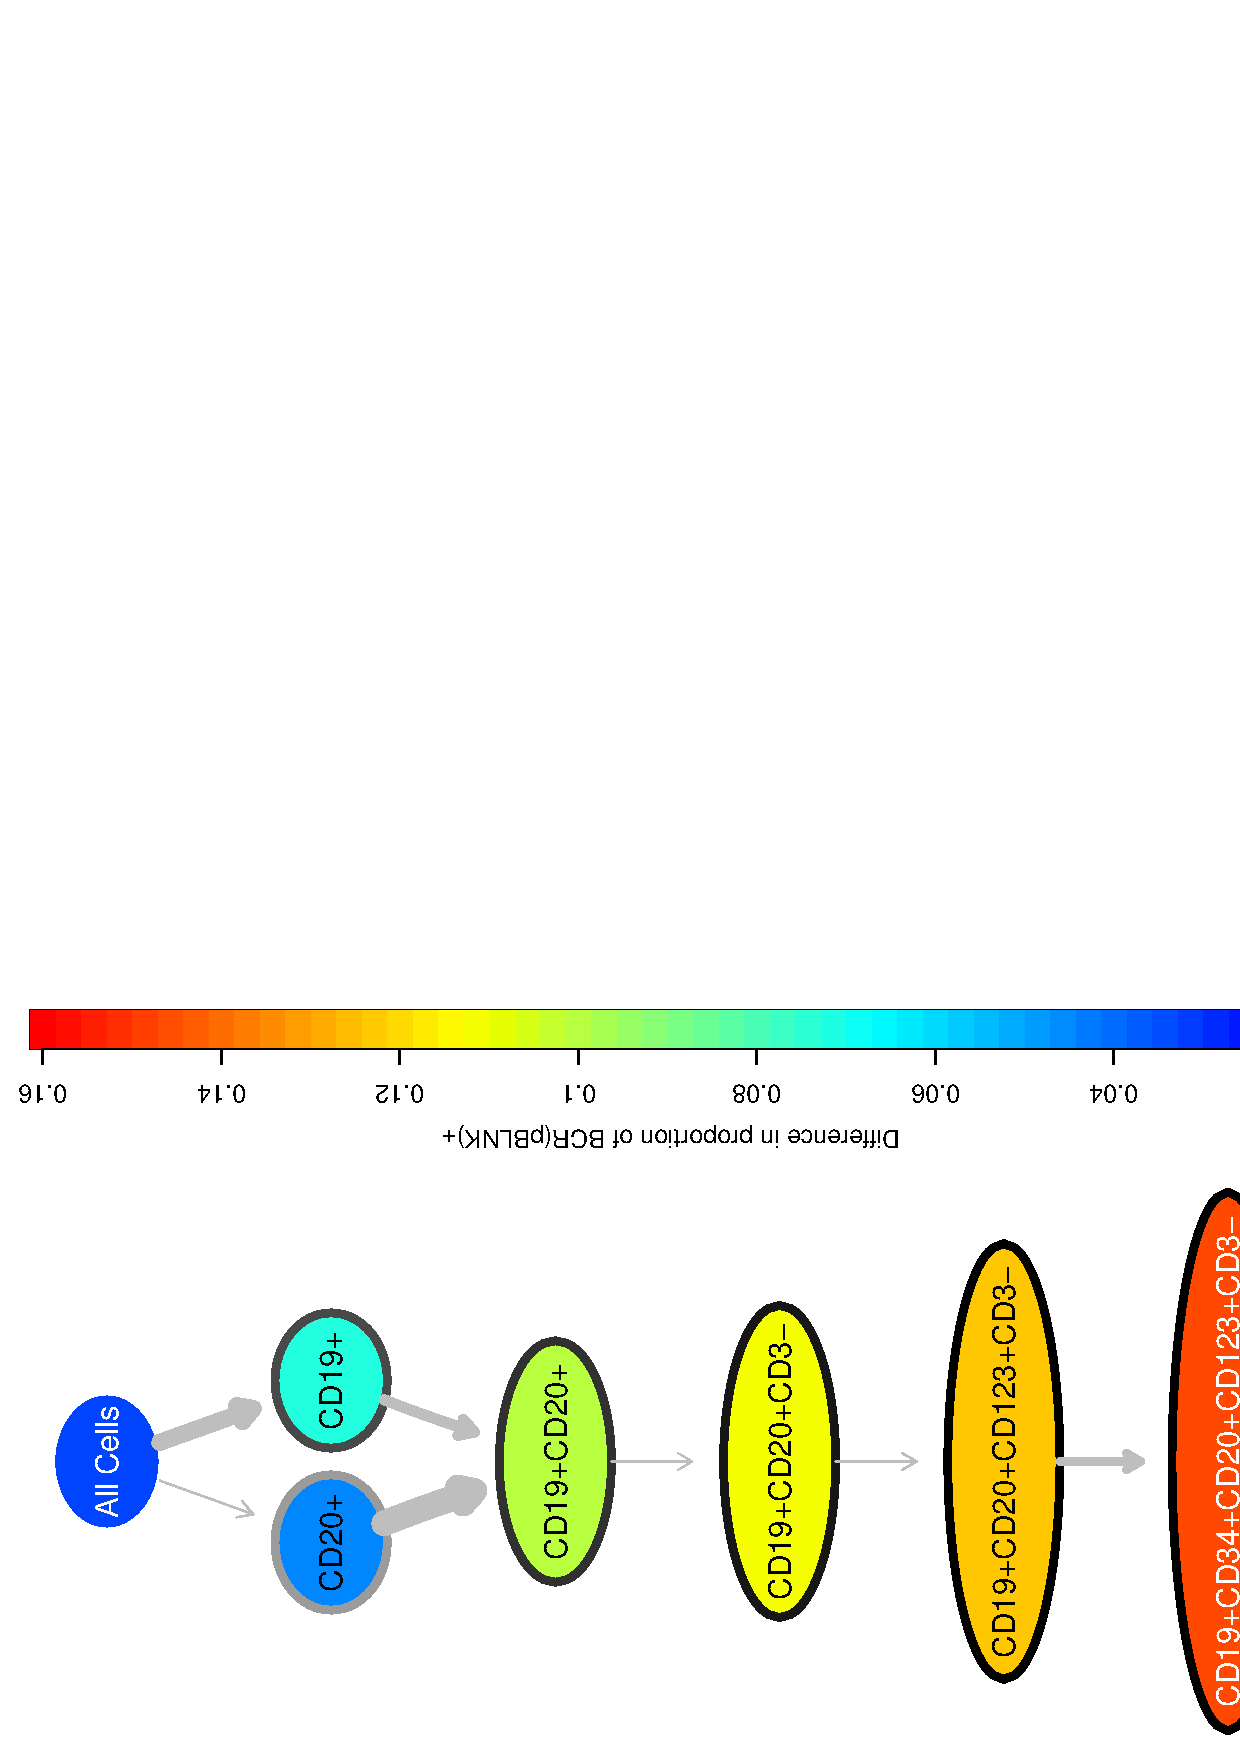
\includegraphics[width=4in,angle=270]{figs/rchy/figs/BCRProportions}&
        \includegraphics[width=4in,angle=270]{figs/rchy/figs/LPSProportions}\\
        (A) IL7 &(B) BCR &(C) LPS\\
      \end{tabular}
    \end{center}
    \caption{Average F-measures of all pairs of results for the cell populations across all samples in the HSCT dataset (\emph{i.e.,} one heatmap for every cell population in the reference).}
    \label{CyTOFProp}
  \end{figure}
  \end{landscape}

  \begin{figure}[!ht]
    \begin{center}
      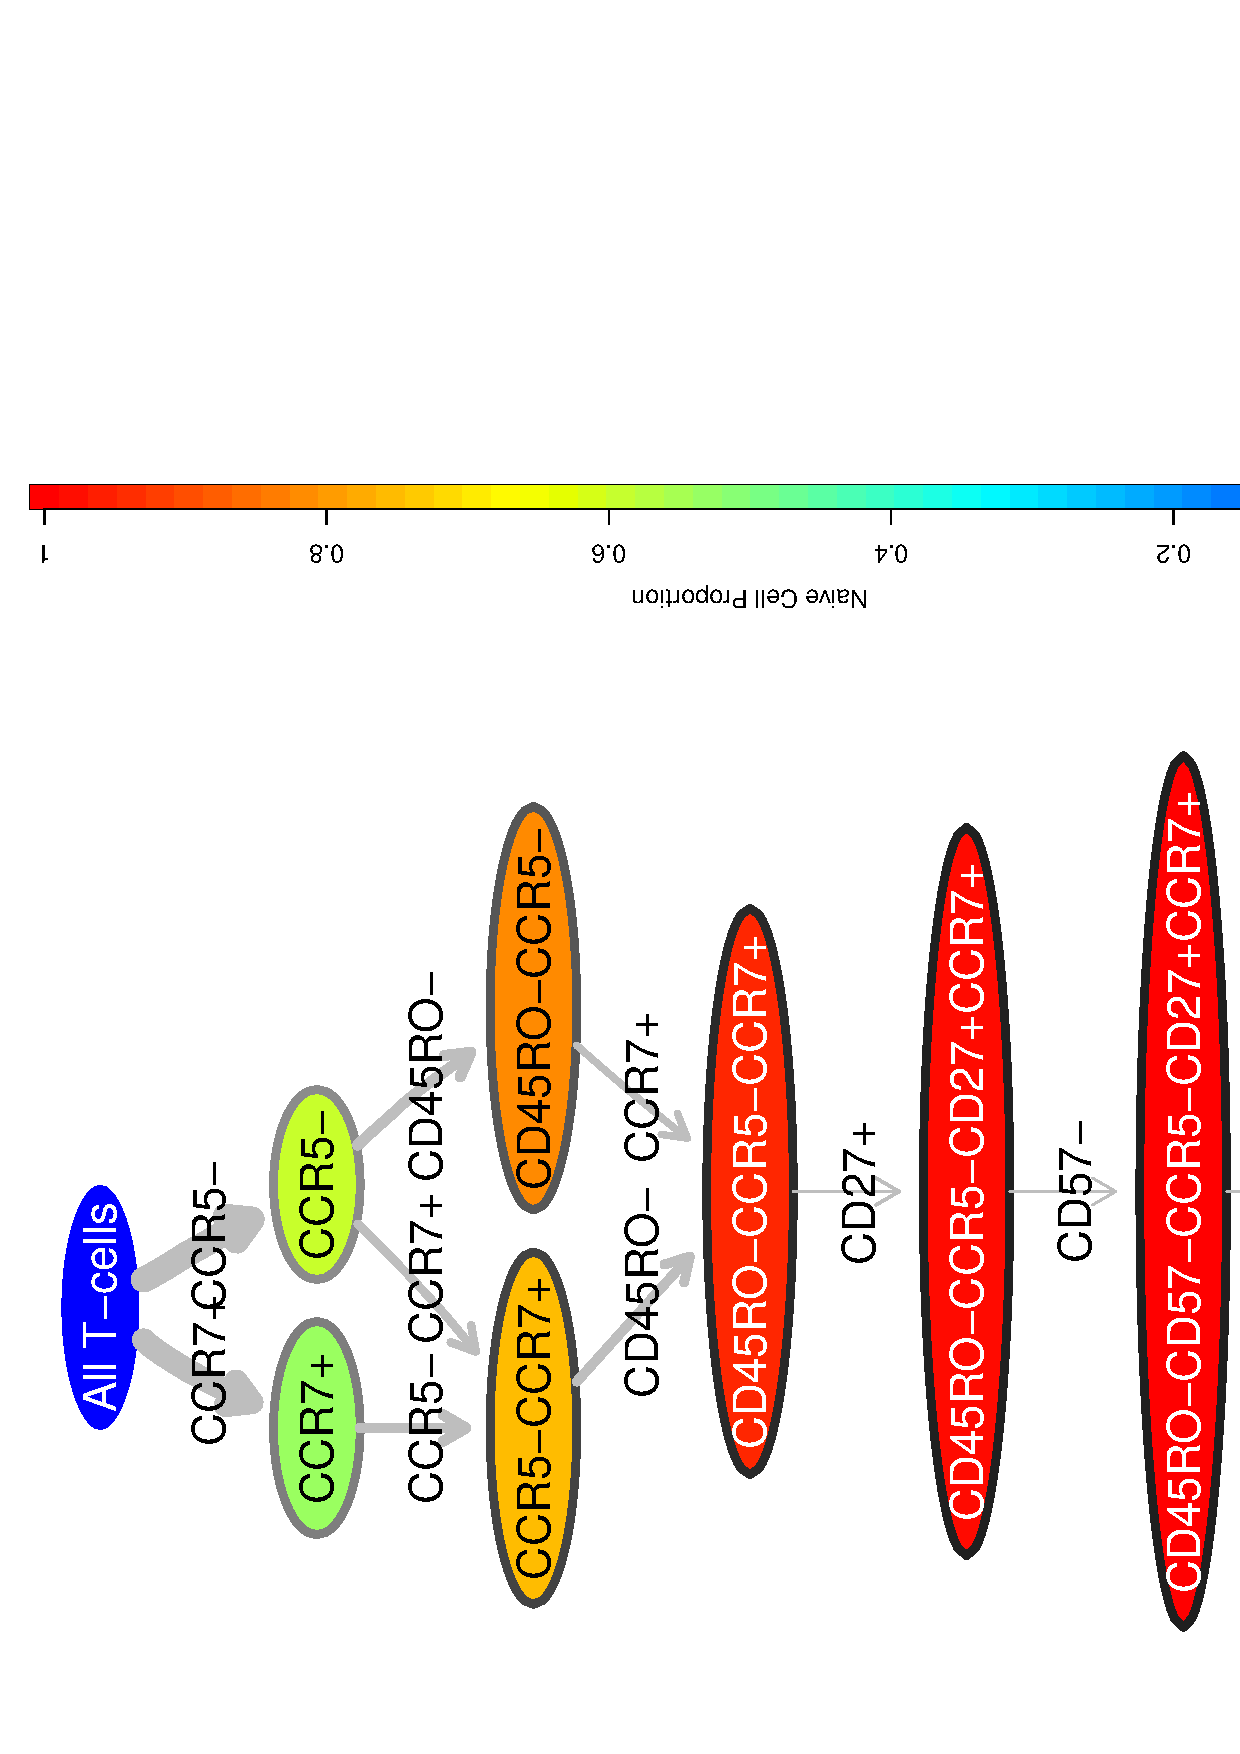
\includegraphics[width=\textwidth, angle=270]{figs/rchy/figs/PropNaiveOverlap}
    \end{center}
    \caption{An optimized cellular hierarchy for identifying naive T-cells. The colour of the nodes and the thickness of the edges shows the purity and change in purity of the original naive phenotype within the given cell population, respectively.
      This is similar to Figure 6 in the main text except the color of the border of the nodes shows the cell proportion of the cell population.
    }
    \label{r1:NaiveOverlapProp}
  \end{figure}

 \begin{figure}[!ht]
    \begin{center}
      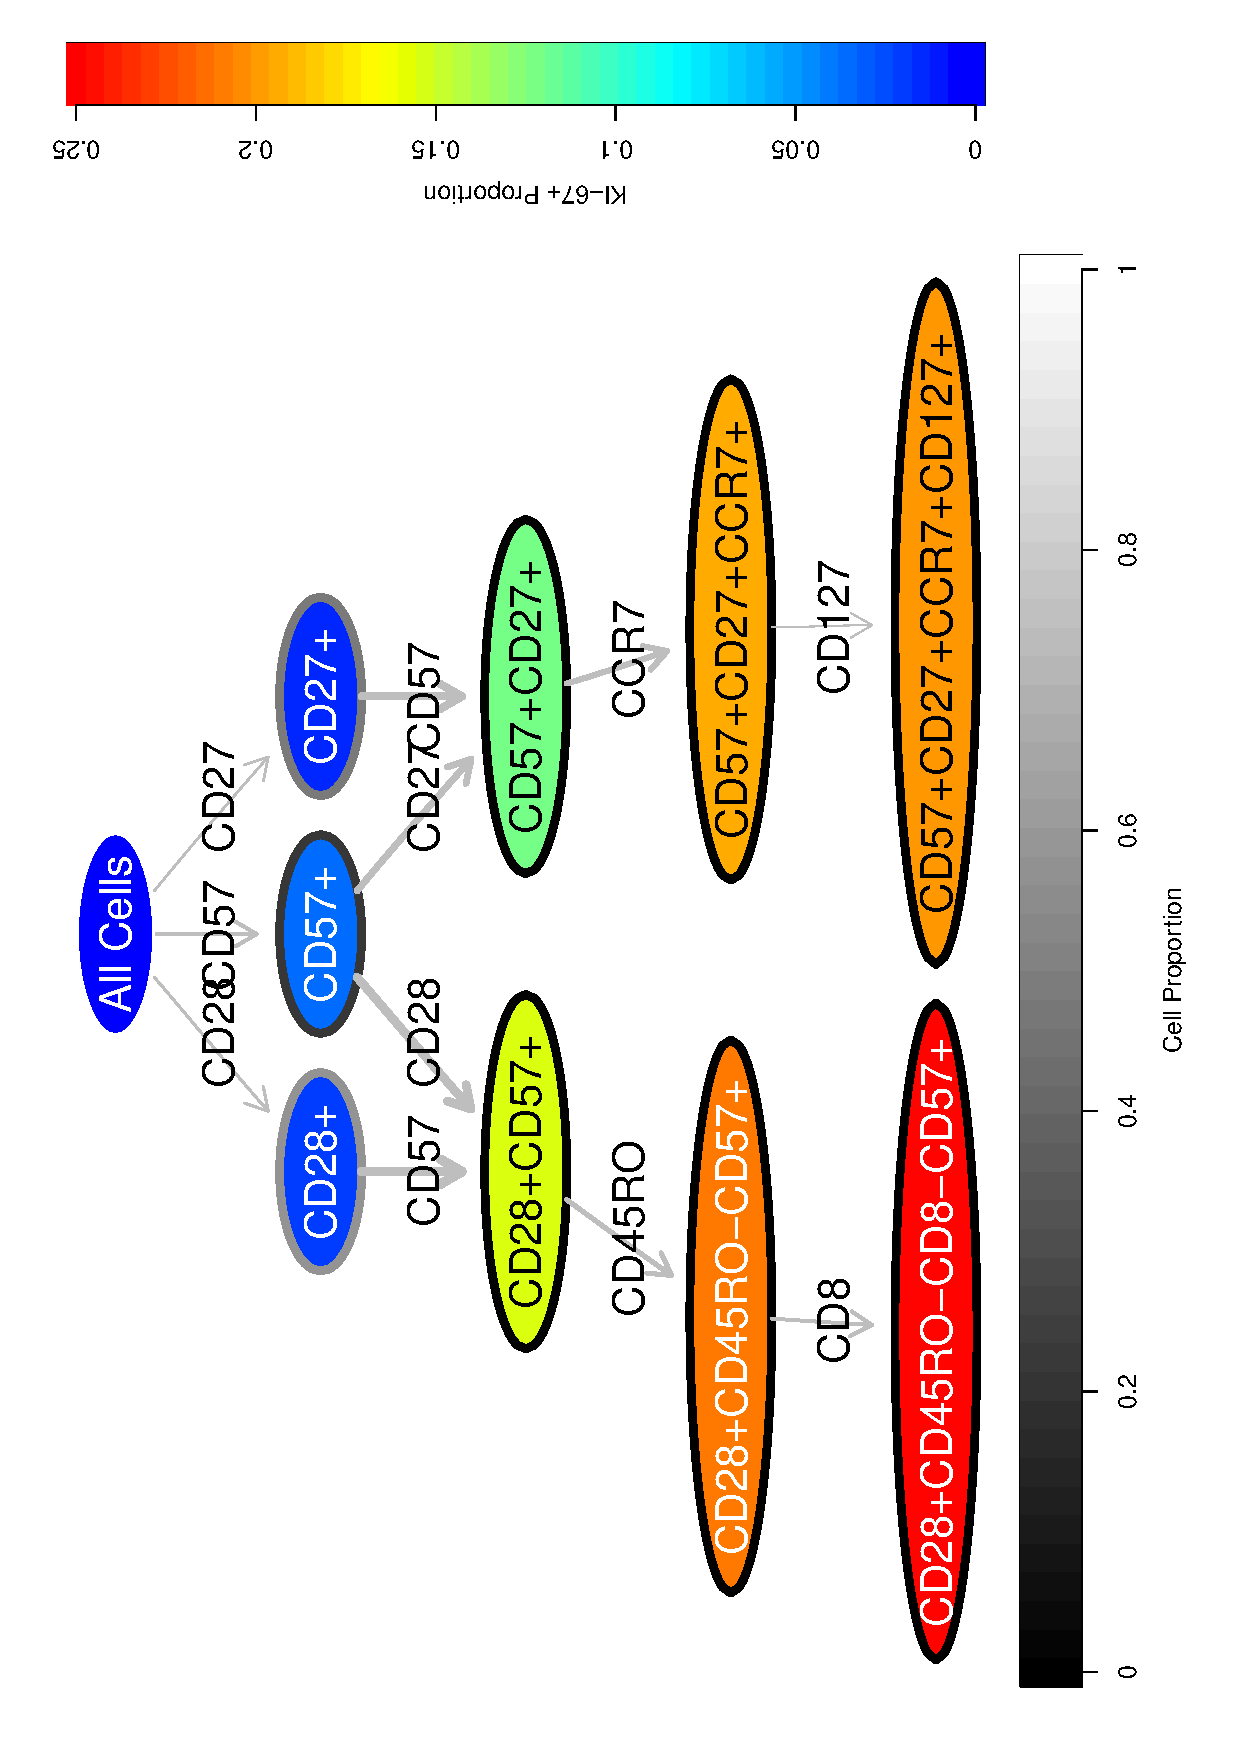
\includegraphics[width=.7\textwidth, angle=270]{figs/rchy/figs/PropKI67Overlap}
    \end{center}
    \caption{A cellular hierarchy for identifying KI-67$^+$ T-cells using surface markers. The colour of the nodes and the thickness of the edges shows the proportion and change in proportion of KI-67$^+$ T-cells, respectively.
      This is similar to Figure 7 in the main text except the color of the border of the nodes shows the cell proportion of the cell population.}
    \label{r1:KI67Overlap}
  \end{figure}

\begin{figure}[!ht]
  \begin{center}
    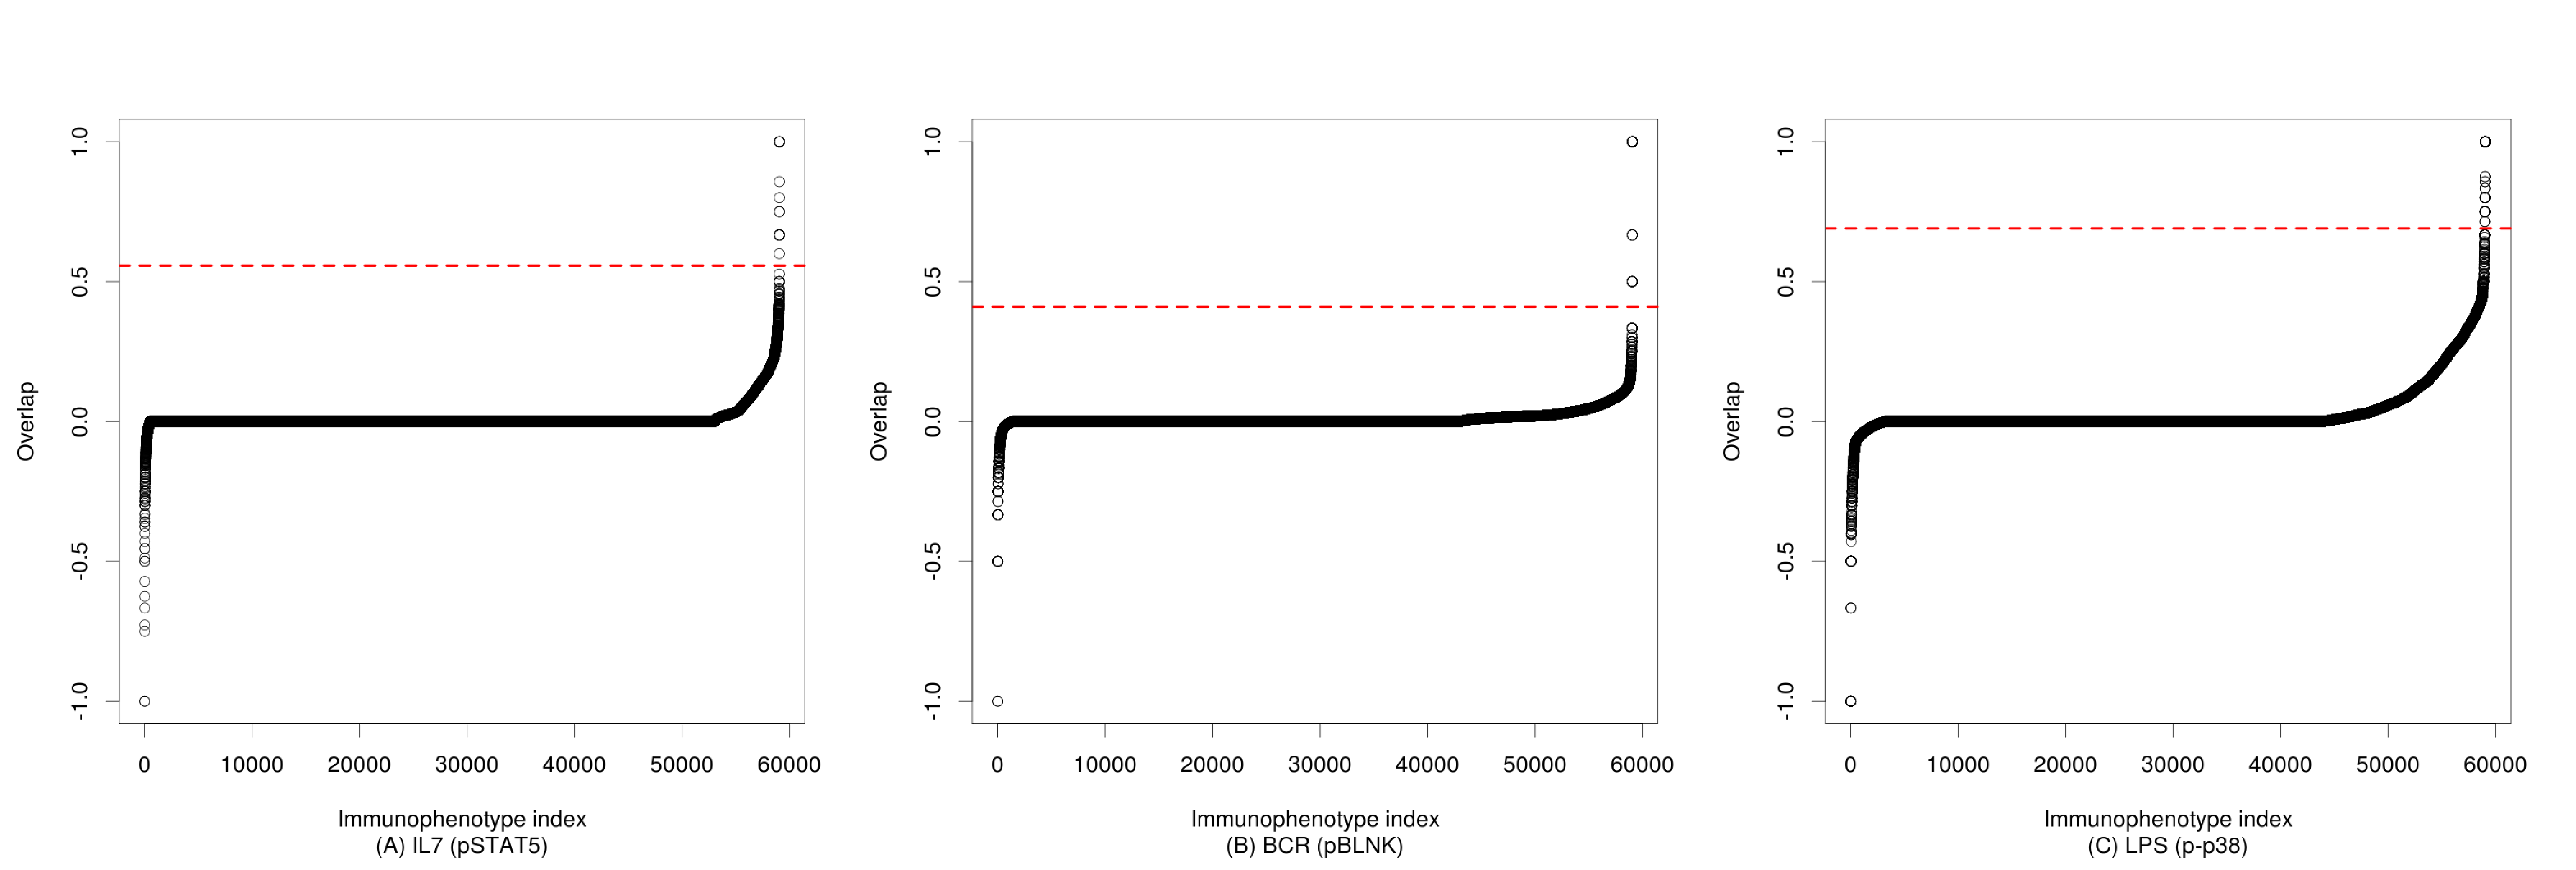
\includegraphics[width=\textwidth]{figs/rchy/figs/overlaps}
  \end{center}
  \caption{All immunophenotypes ordered by their overlap with the cell population of interest. The red dashed lines indicate the cutoffs used for selecting the immunophenotypes with ``high overlap''.}
  \label{r1:overlaps}
\end{figure}


\begin{figure}[!ht]
  \begin{center}
    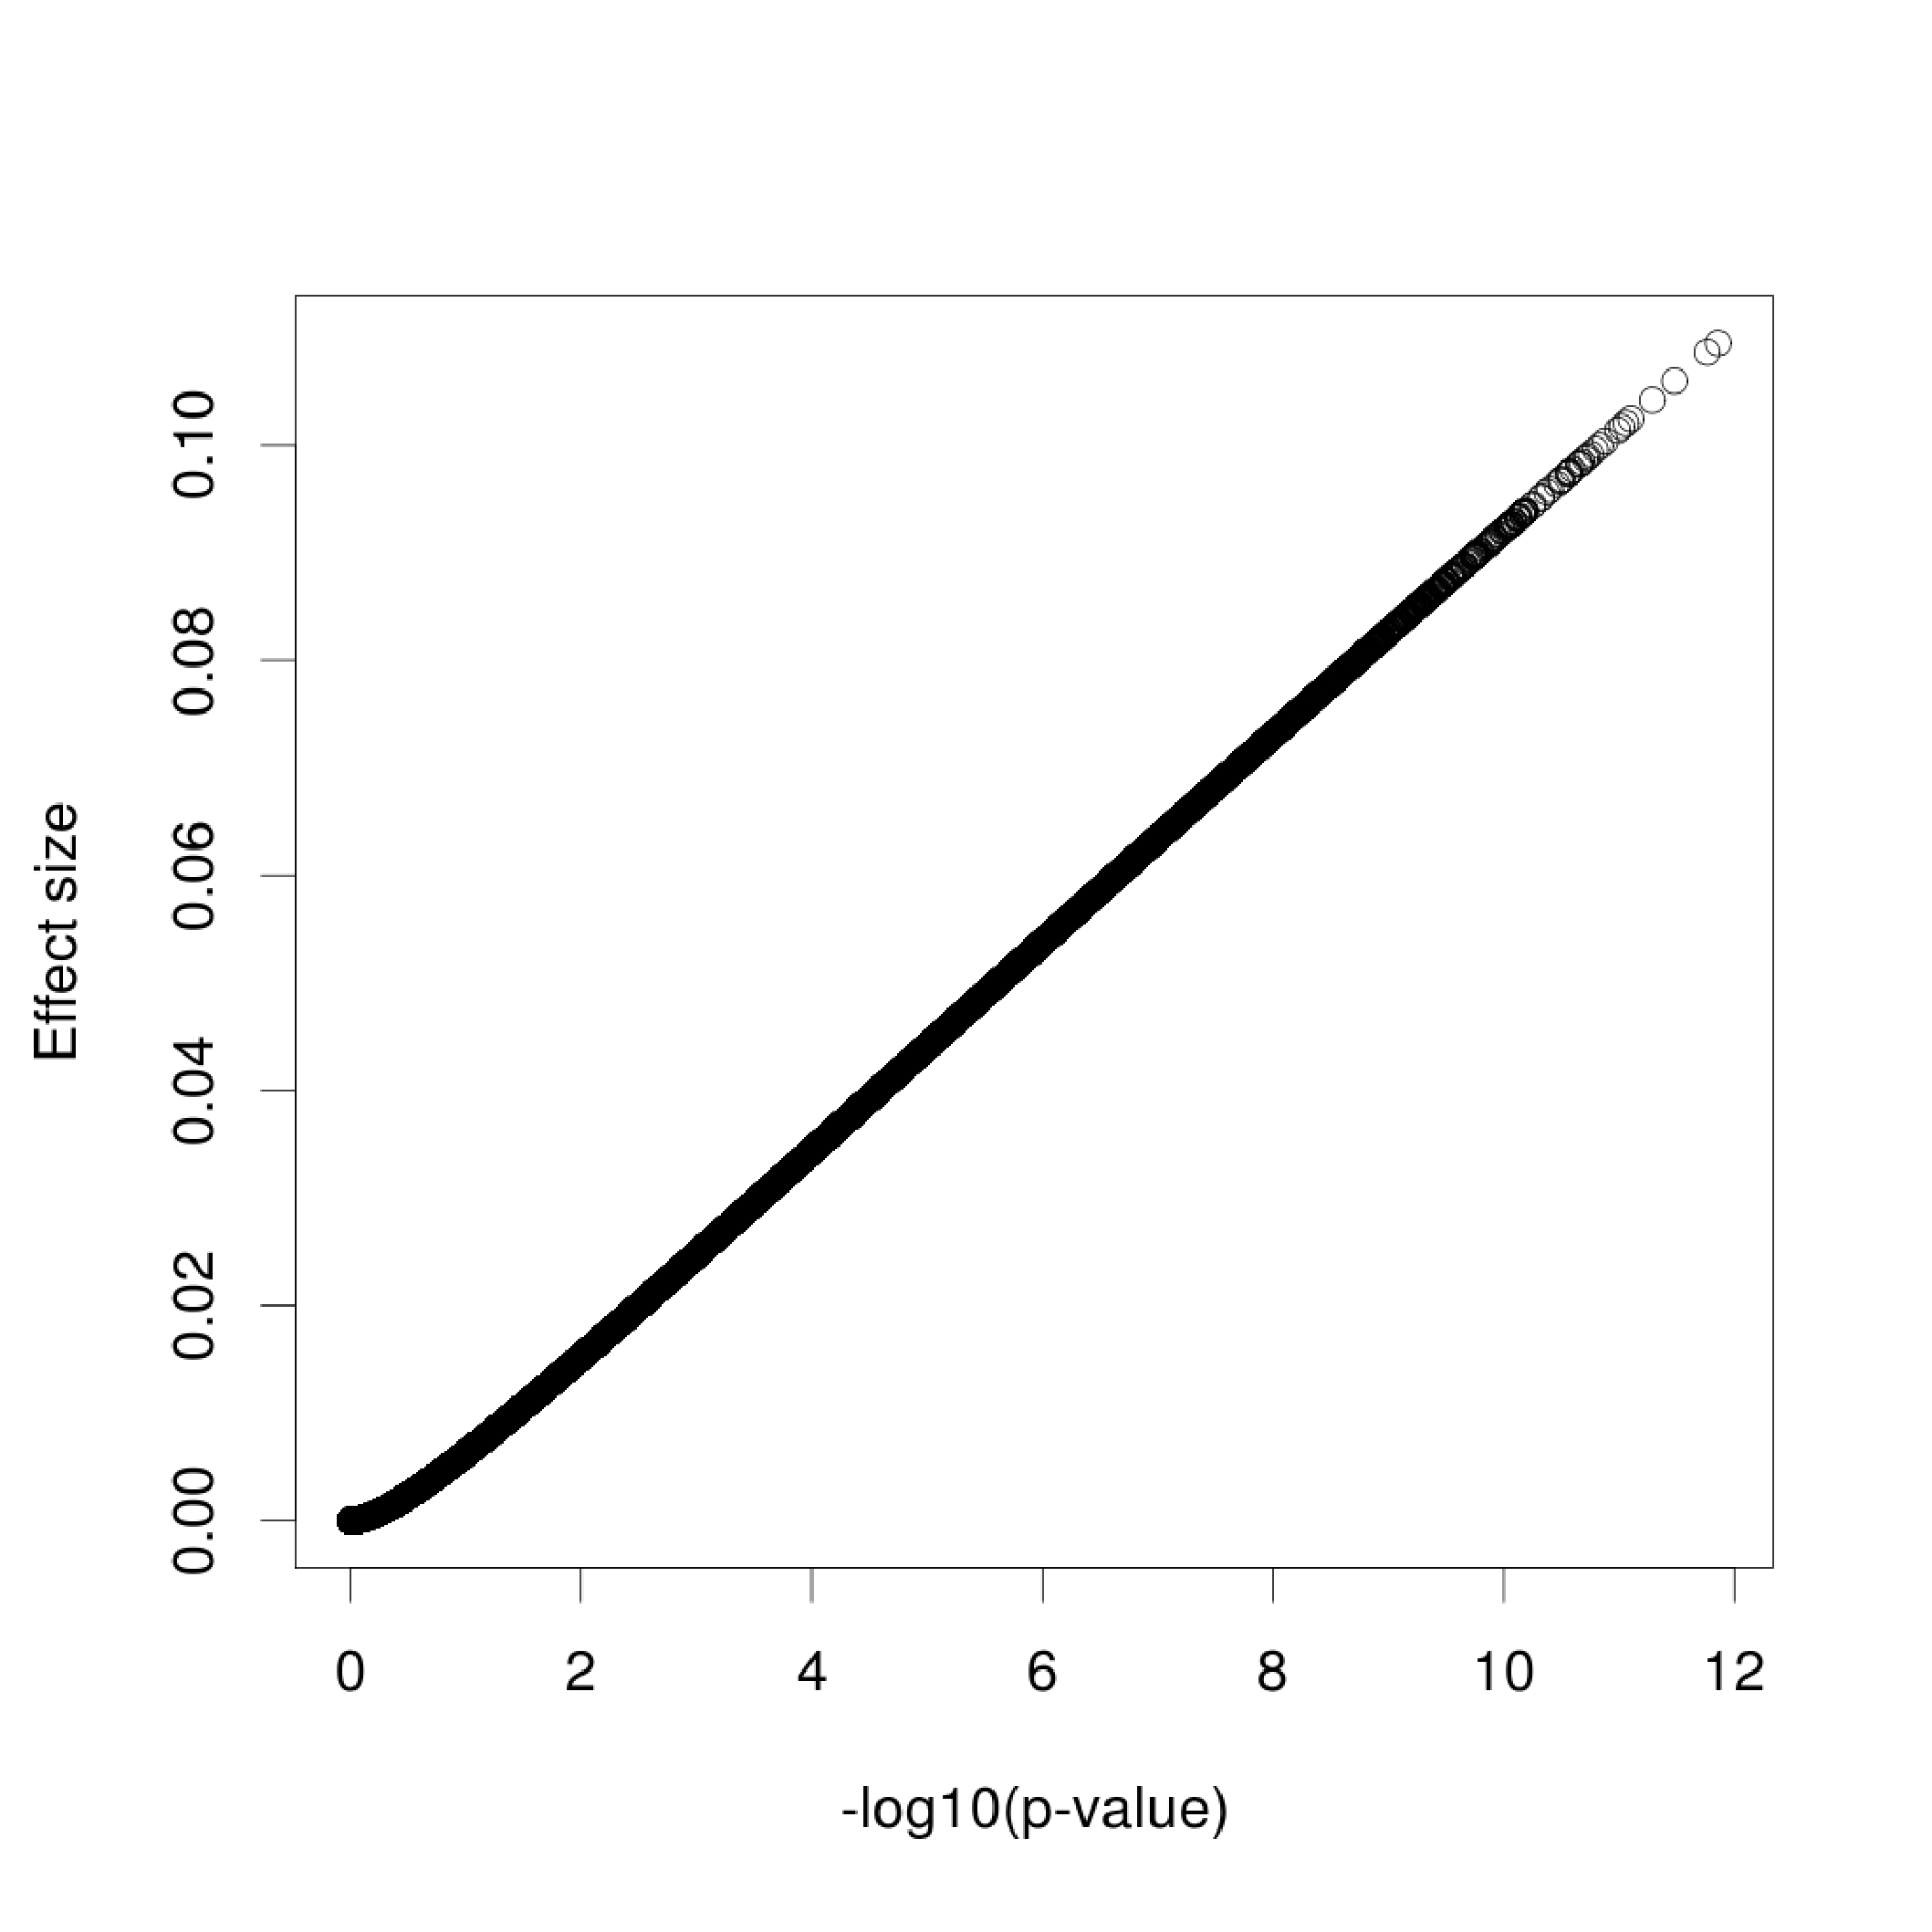
\includegraphics[width=10cm]{figs/rchy/figs/cor}
  \end{center}
  \caption{The correlation between the effect sizes and p-values of the log rank tests for the Cox proportional hazards models for each immunophenotype. The Pearson correlation coefficient was determined as $0.997$, indicating a highly significant correlation with a p-value  $< 2.2 \times 10^{-16}$.}
  \label{r1:effectsizevspv}
\end{figure}


\section{Lymphoma Diagnosis Quality Checking}
